\chapter*{LAMPIRAN}
\addcontentsline{toc}{chapter}{LAMPIRAN}
\stepcounter{chapter}
\renewcommand{\thefigure}{6.\arabic{figure}}
\setcounter{figure}{0}

\section*{Lampiran 1: Kode Program Python Pengenalan SIBI Berbasis MediaPipe dan Model DNN}
\addcontentsline{toc}{section}{Lampiran 1: Kode Program Python Pengenalan SIBI Berbasis MediaPipe dan Model DNN}

Program berikut merupakan implementasi nyata akuisisi citra kamera secara \textit{real-time}, ekstraksi 21 titik persendian tangan menggunakan MediaPipe Hands, serta inferensi klasifikasi abjad SIBI menggunakan model \textit{Deep Neural Network} (DNN) \texttt{.keras} dan visualisasi GUI Tkinter.

\begin{lstlisting}[language=Python, caption={Implementasi Program Python untuk Mode Pengenalan SIBI pada meArm}]
import cv2
import numpy as np
import tensorflow as tf
import mediapipe as mp
import tkinter as tk
from PIL import Image, ImageTk
import joblib

# Pemuatan Model DNN dan Label Encoder
model = tf.keras.models.load_model("model/sibi_model.keras")
label_encoder = joblib.load("model/label_encoder.pkl")
labels = list(label_encoder.classes_)

# Inisialisasi MediaPipe Hands
mp_hands = mp.solutions.hands
hands = mp_hands.Hands(
    static_image_mode=False,
    max_num_hands=1,
    min_detection_confidence=0.9,
    min_tracking_confidence=0.9
)
mp_draw = mp.solutions.drawing_utils

class SIBIGUI:
    def __init__(self, root):
        self.root = root
        root.title("SIBI Detector - MediaPipe Mode")
        root.geometry("1000x700")

        self.cam_label = tk.Label(root, bg="black")
        self.cam_label.pack(pady=5)
        self.info_label = tk.Label(root, text="Huruf Terdeteksi: -", font=("Arial", 14), fg="#00ff00")
        self.info_label.pack(pady=5)

        self.cap = cv2.VideoCapture(0)
        self.current_char = ""
        self.update_frame()

    def update_frame(self):
        ret, frame = self.cap.read()
        if ret:
            frame = cv2.flip(frame, 1)
            rgb_frame = cv2.cvtColor(frame, cv2.COLOR_BGR2RGB)

            # Deteksi Landmark Tangan
            results = hands.process(rgb_frame)
            if results.multi_hand_landmarks:
                for hand_landmarks in results.multi_hand_landmarks:
                    mp_draw.draw_landmarks(
                        frame, hand_landmarks, mp_hands.HAND_CONNECTIONS,
                        mp_draw.DrawingSpec(color=(0, 255, 0), thickness=2, circle_radius=2),
                        mp_draw.DrawingSpec(color=(0, 0, 255), thickness=2)
                    )

                    # Ekstraksi 21 Titik Koordinat Spasial (x, y, z)
                    landmarks = []
                    for lm in hand_landmarks.landmark:
                        landmarks.extend([lm.x, lm.y, lm.z])

                    # Inferensi Model DNN
                    prediction = model.predict(np.array([landmarks]), verbose=0)
                    class_id = np.argmax(prediction)
                    self.current_char = labels[class_id]
                    self.info_label.config(text=f"Huruf Terdeteksi: {self.current_char}")

            img = Image.fromarray(cv2.cvtColor(frame, cv2.COLOR_BGR2RGB))
            imgtk = ImageTk.PhotoImage(image=img)
            self.cam_label.imgtk = imgtk
            self.cam_label.config(image=imgtk)

        self.root.after(10, self.update_frame)

if __name__ == "__main__":
    root = tk.Tk()
    app = SIBIGUI(root)
    root.mainloop()
\end{lstlisting}

\newpage
\section*{Lampiran 2: Kode Program Python Teleoperasi Dinamis Dobot Magician}
\addcontentsline{toc}{section}{Lampiran 2: Kode Program Python Teleoperasi Dinamis Dobot Magician}

Program berikut memetakan posisi spasial tangan operator secara \textit{real-time} ke koordinat kerja 3D Dobot Magician melalui pustaka \texttt{pydobotplus}, dilengkapi filter penghalusan gerak (\textit{exponential smoothing}), ambang batas pemindahan (\textit{anti-spam threshold}), serta logika kendali \textit{suction cup} berbasis gestur jepit ibu jari dan telunjuk.

\begin{lstlisting}[language=Python, caption={Implementasi Program Python untuk Teleoperasi Dobot Magician}]
import cv2
import mediapipe as mp
from pydobotplus import Dobot
import math

MAX_RADIUS = 310.0      # Batas jangkauan kerja robot (mm)
LIMIT_Z_MIN = -50.0     # Batas tinggi minimum (mm)
LIMIT_Z_MAX = 150.0     # Batas tinggi maksimum (mm)

SMOOTHING = 0.2         # Bobot filter penghalusan gerak
MOVE_THRESHOLD = 5.0    # Ambang batas gerak minimum anti-spam (mm)

class DobotTeleoperation:
    def __init__(self, port="COM3"):
        self.device = Dobot(port=port)
        self.curr_x, self.curr_y, self.curr_z = 200.0, 0.0, 0.0
        self.last_x, self.last_y, self.last_z = 200.0, 0.0, 0.0
        self.grip_state = False

        self.mp_hands = mp.solutions.hands
        self.hands = self.mp_hands.Hands(
            max_num_hands=1,
            min_detection_confidence=0.7,
            min_tracking_confidence=0.5
        )
        self.mp_draw = mp.solutions.drawing_utils

    def check_limit(self, x, y, z):
        radius = math.sqrt(x**2 + y**2)
        return radius <= MAX_RADIUS and LIMIT_Z_MIN <= z <= LIMIT_Z_MAX

    def process_hand_tracking(self, frame):
        img_h, img_w, _ = frame.shape
        rgb_frame = cv2.cvtColor(frame, cv2.COLOR_BGR2RGB)
        results = self.hands.process(rgb_frame)

        if results.multi_hand_landmarks:
            for hand_lms in results.multi_hand_landmarks:
                self.mp_draw.draw_landmarks(frame, hand_lms, self.mp_hands.HAND_CONNECTIONS)

                lm_wrist = hand_lms.landmark[0]
                lm_mid = hand_lms.landmark[9]

                # Pemetaan Koordinat Citra ke Ruang Cartesian Robot
                target_y = (lm_mid.x - 0.5) * 450.0             # Sumbu Y (Kiri-Kanan)
                target_z = (1.0 - lm_mid.y) * 220.0 - 50.0      # Sumbu Z (Naik-Turun)

                # Estimasi Kedalaman Sumbu X berbasis Skala Ukuran Tangan
                hand_size = abs(lm_wrist.y - lm_mid.y)
                target_x = 180.0 + (hand_size - 0.1) * 600.0
                target_x = max(180.0, min(target_x, 305.0))

                # Penghalusan Gerak (Exponential Smoothing)
                self.curr_x = self.curr_x * (1 - SMOOTHING) + target_x * SMOOTHING
                self.curr_y = self.curr_y * (1 - SMOOTHING) + target_y * SMOOTHING
                self.curr_z = self.curr_z * (1 - SMOOTHING) + target_z * SMOOTHING

                # Logika Anti-Spam: Pengiriman instruksi jika delta gerak > 5 mm
                dist = math.sqrt((self.curr_x - self.last_x)**2 +
                                 (self.curr_y - self.last_y)**2 +
                                 (self.curr_z - self.last_z)**2)

                if dist > MOVE_THRESHOLD and self.check_limit(self.curr_x, self.curr_y, self.curr_z):
                    try:
                        self.device.move_to(x=self.curr_x, y=self.curr_y, z=self.curr_z, r=0, wait=False)
                        self.last_x, self.last_y, self.last_z = self.curr_x, self.curr_y, self.curr_z
                    except Exception as e:
                        print("Koneksi Error:", e)

                # Logika Jepit Gripper / Suction (Jarak Euclidean Ujung Telunjuk - Ibu Jari)
                x4, y4 = hand_lms.landmark[4].x * img_w, hand_lms.landmark[4].y * img_h
                x8, y8 = hand_lms.landmark[8].x * img_w, hand_lms.landmark[8].y * img_h
                is_fist = math.hypot(x8 - x4, y8 - y4) < 30.0

                if is_fist != self.grip_state:
                    self.grip_state = is_fist
                    self.device.suck(enable=self.grip_state)
\end{lstlisting}

\newpage
\section*{Lampiran 3: Kode Program Firmware Arduino Kendali Kinematika Balikan meArm}
\addcontentsline{toc}{section}{Lampiran 3: Kode Program Firmware Arduino Kendali Kinematika Balikan meArm}

Program berikut merupakan firmware mikrokontroler Arduino yang mengimplementasikan perhitungan trigonometri \textit{Inverse Kinematics} (IK) untuk mengonversi target koordinat spasial Cartesian $(X,Y,Z)$ menjadi sudut rotasi 4 motor servo meArm secara halus (\textit{smooth sequential movement}).

\begin{lstlisting}[language=C++, caption={Implementasi Program Arduino Kinematika Balikan meArm 4-DOF}]
#include <Servo.h>
#include <math.h>

const float L1 = 90.0; // Panjang tautan lengan atas (mm)
const float L2 = 90.0; // Panjang tautan lengan bawah (mm)

#define PIN_B 3 // Servo Basis
#define PIN_S 5 // Servo Bahu (Shoulder)
#define PIN_E 6 // Servo Siku (Elbow)
#define PIN_G 9 // Servo Gripper

Servo svB, svS, svE, svG;
int posB = 75, posS = 85, posE = 54, posG = 180;

void setup() {
  Serial.begin(115200);
  svB.attach(PIN_B); svS.attach(PIN_S);
  svE.attach(PIN_E); svG.attach(PIN_G);
  svB.write(posB); svS.write(posS);
  svE.write(posE); svG.write(posG);
}

void moveSmooth(Servo &sv, int &pos, int target, int delayMs = 15) {
  target = constrain(target, 0, 180);
  if (pos == target) return;
  int step = (target > pos) ? 1 : -1;
  while (pos != target) {
    pos += step;
    sv.write(pos);
    delay(delayMs);
  }
}

// Komputasi Kinematika Balikan (Inverse Kinematics)
void executeXYZ(float x, float y, float z) {
  float radBase = atan2(y, x);
  float degBase = radBase * 180.0 / PI;

  float r = sqrt(x * x + y * y);
  float d = sqrt(r * r + z * z);
  if (d > (L1 + L2)) return; // Batas fisik jangkauan link robot

  float alpha1 = atan2(z, r);
  float cosAlpha2 = (L1 * L1 + d * d - L2 * L2) / (2.0 * L1 * d);
  float alpha2 = acos(constrain(cosAlpha2, -1.0, 1.0));
  float thetaShoulder = (alpha1 + alpha2) * 180.0 / PI;

  float cosBeta = (L1 * L1 + L2 * L2 - d * d) / (2.0 * L1 * L2);
  float beta = acos(constrain(cosBeta, -1.0, 1.0));
  float thetaElbow = beta * 180.0 / PI;

  moveSmooth(svB, posB, degBase);
  moveSmooth(svS, posS, thetaShoulder);
  moveSmooth(svE, posE, thetaElbow);
}

void loop() {
  if (Serial.available() > 0) {
    char cmd = Serial.read();
    if (cmd == 'A') executeXYZ(80, 0, 40);
    else if (cmd == 'B') executeXYZ(60, 60, 30);
    else if (cmd == 'C') moveSmooth(svG, posG, 90);  // Tutup Gripper
    else if (cmd == 'D') moveSmooth(svG, posG, 180); // Buka Gripper
  }
}
\end{lstlisting}

\newpage
\section*{Lampiran 4: Dokumentasi Perangkat Keras dan Pengujian Robot}
\addcontentsline{toc}{section}{Lampiran 4: Dokumentasi Perangkat Keras dan Pengujian Robot}

Dokumentasi visual berikut memuat seluruh dokumentasi perangkat keras, perakitan, dan proses pengujian eksperimental untuk kedua platform lengan robot (meArm 4-DOF dan Dobot Magician) yang diperoleh selama pelaksanaan kegiatan di laboratorium:

\subsection*{4.1 Dokumentasi Purwarupa dan Pengujian Lengan Robot meArm}

\begin{figure}[htbp]
    \centering
    \begin{subfigure}[b]{0.48\textwidth}
        \centering
        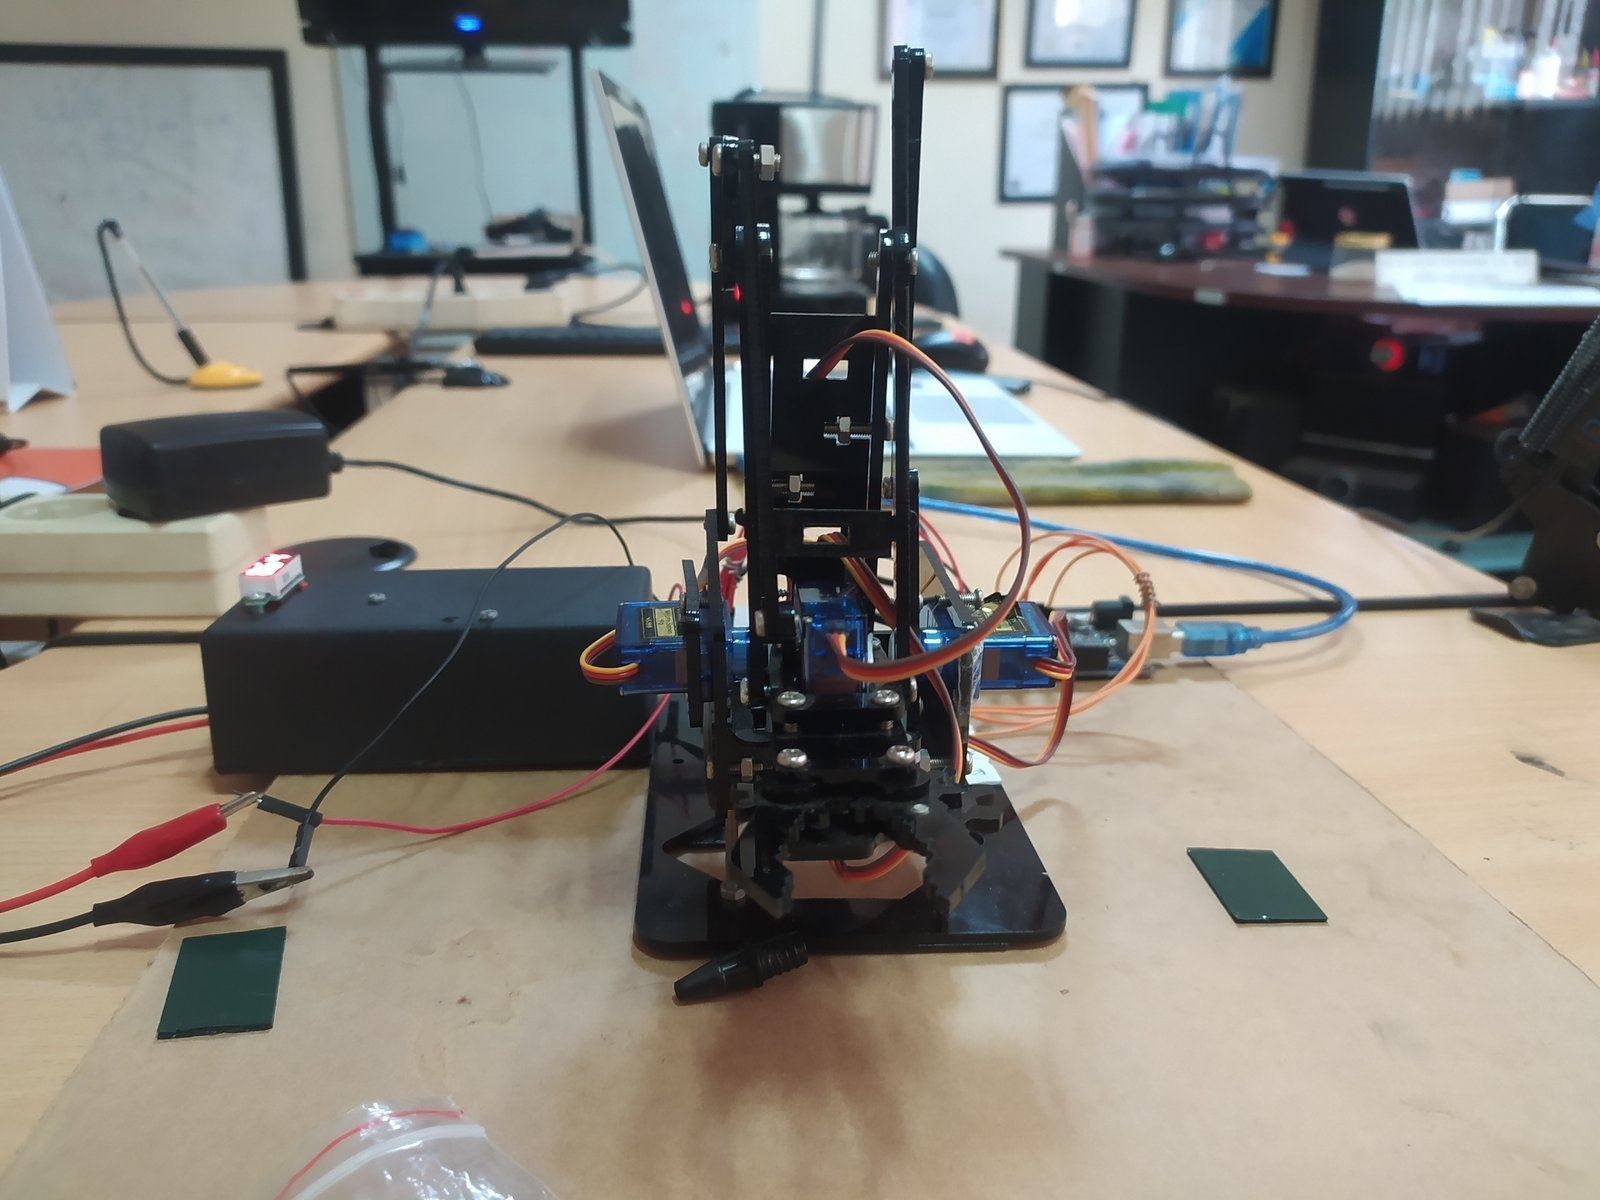
\includegraphics[width=\textwidth]{Gambar/Gambar6_1_mearm_tampak_depan.jpg}
        \caption{Purwarupa meArm (Tampak Depan)}
        \label{fig:app_6_1}
    \end{subfigure}
    \hfill
    \begin{subfigure}[b]{0.48\textwidth}
        \centering
        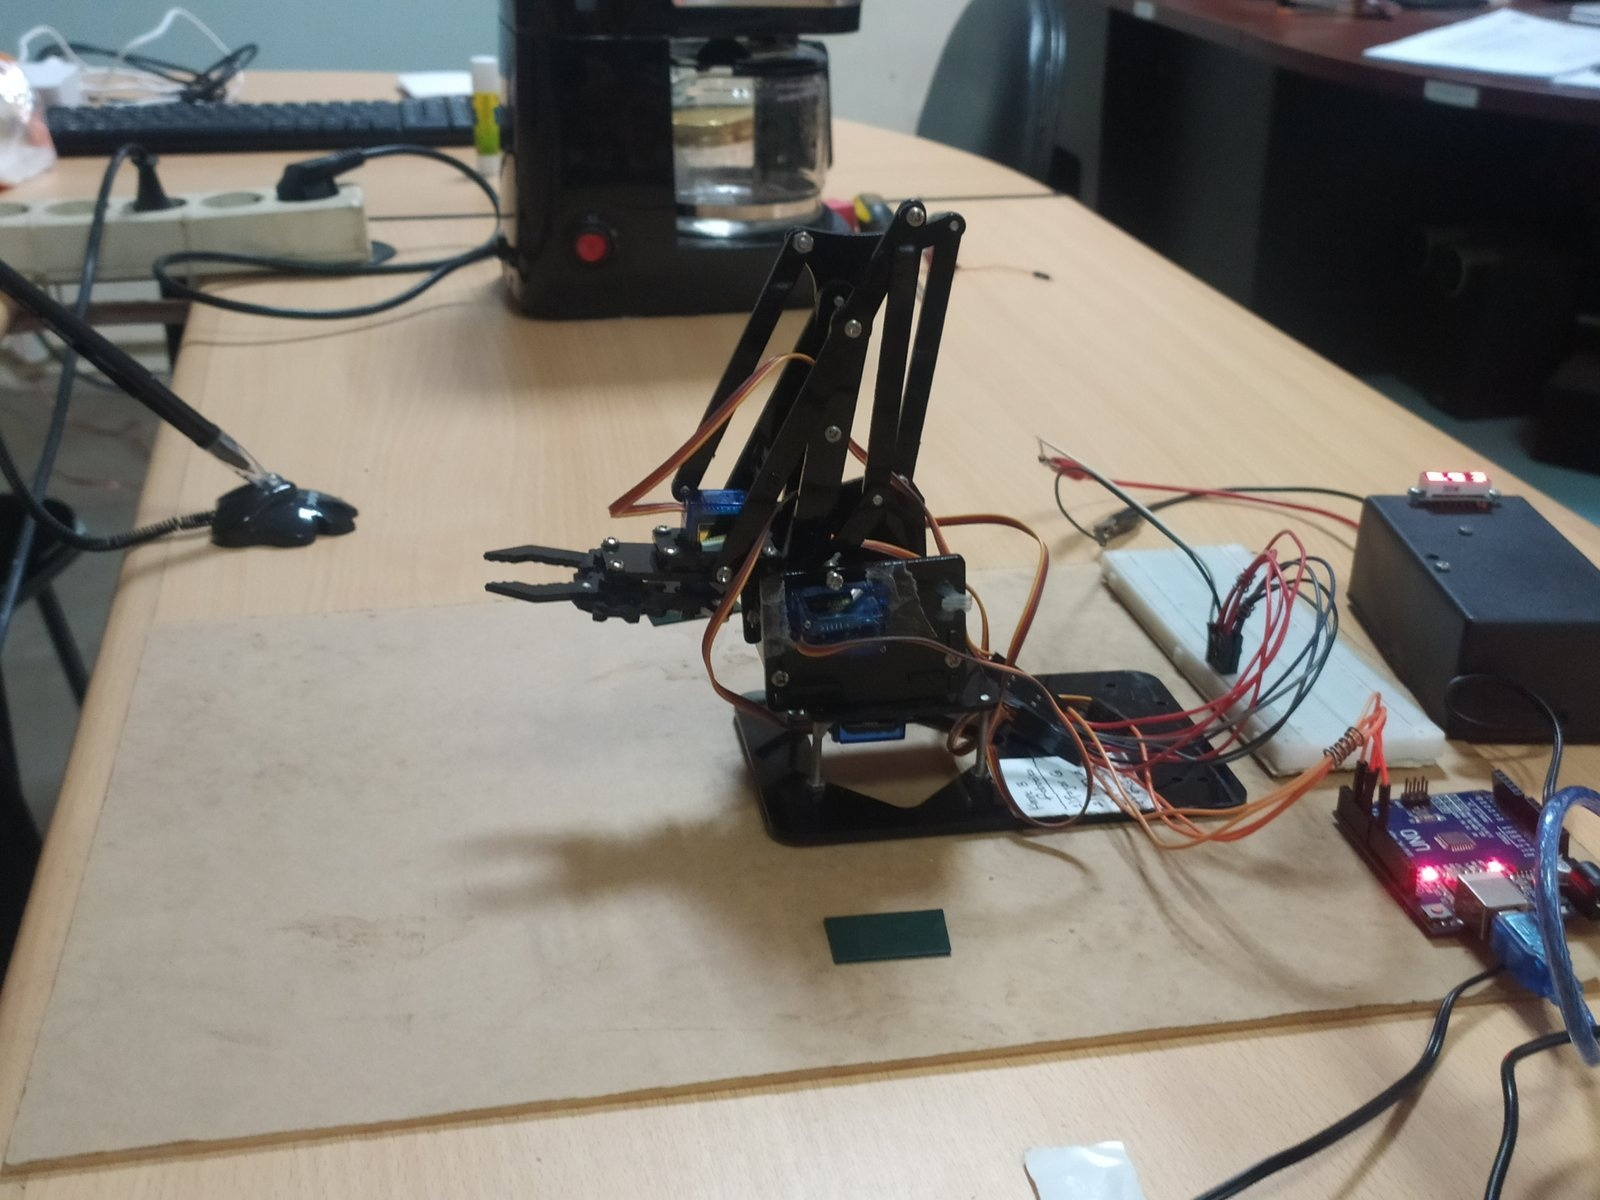
\includegraphics[width=\textwidth]{Gambar/Gambar6_2_mearm_dan_mikrokontroler.jpg}
        \caption{meArm dan Mikrokontroler}
        \label{fig:app_6_2}
    \end{subfigure}
    \caption{Dokumentasi Fisik Purwarupa meArm 4-DOF}
\end{figure}

\begin{figure}[htbp]
    \centering
    \begin{subfigure}[b]{0.48\textwidth}
        \centering
        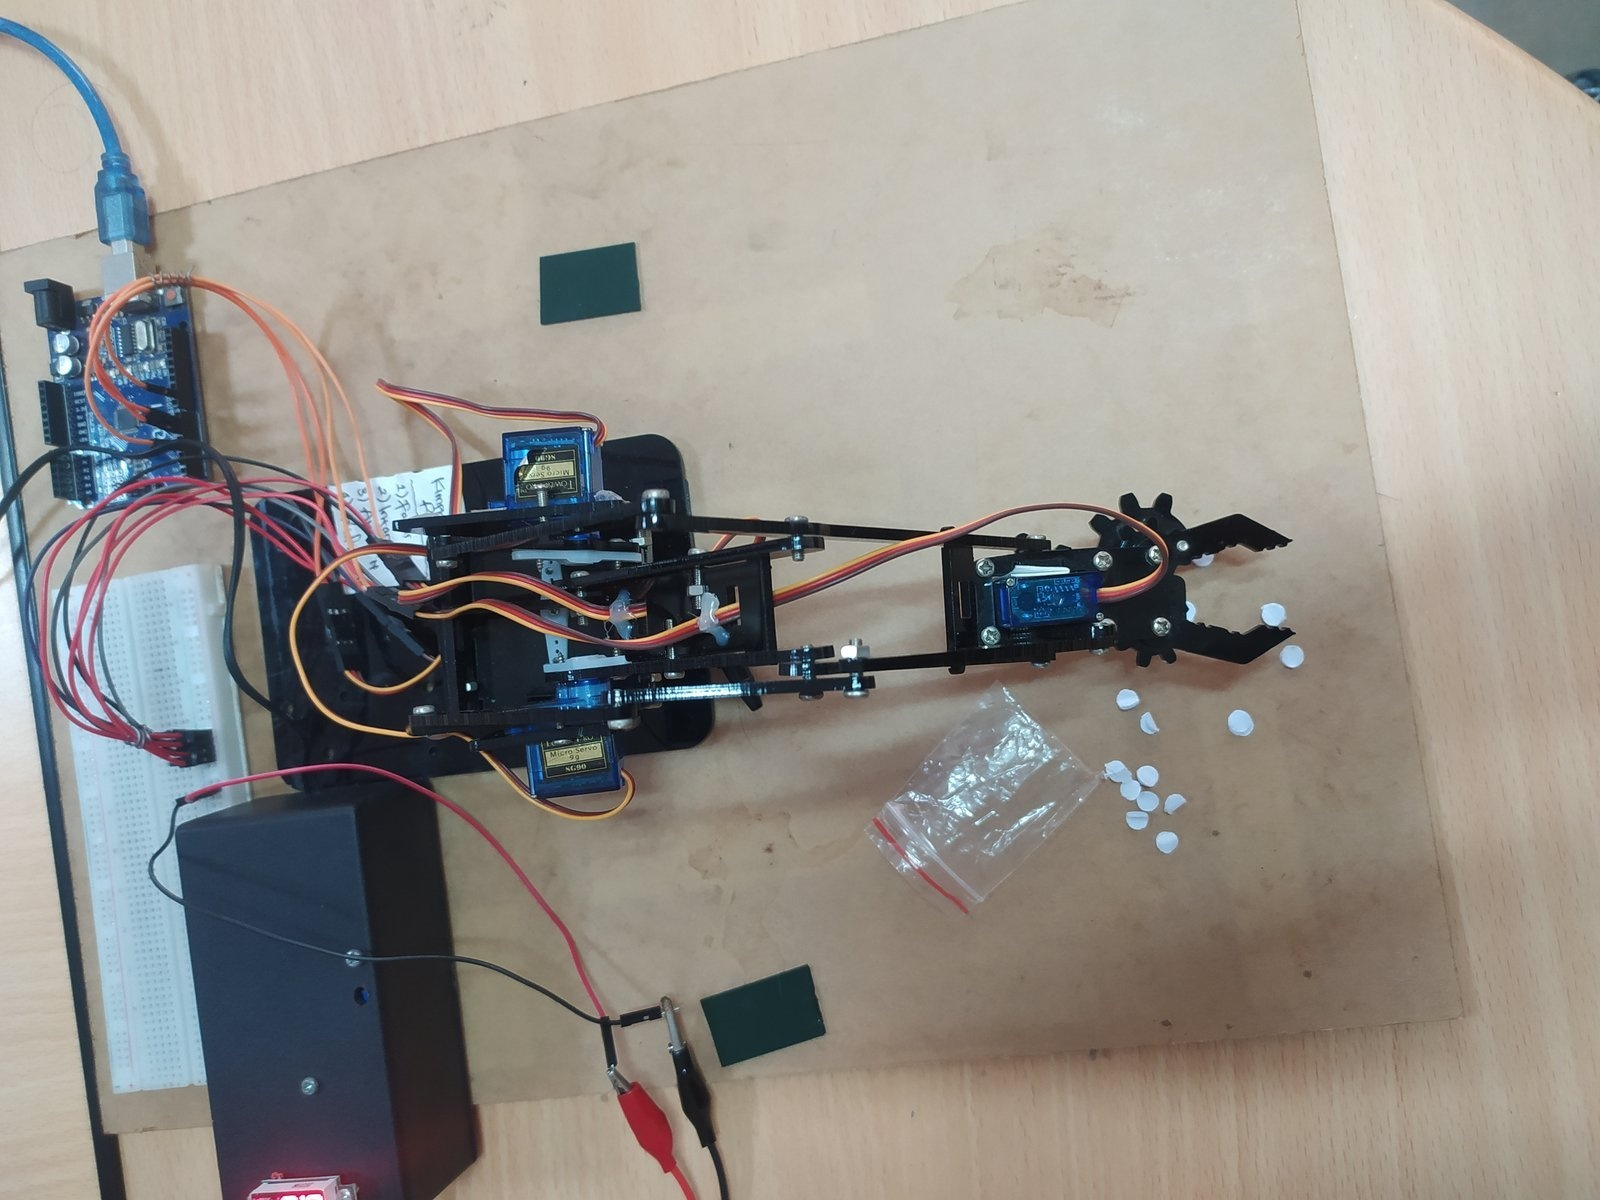
\includegraphics[width=\textwidth]{Gambar/Gambar6_3_mearm_tampak_atas.jpg}
        \caption{Purwarupa meArm (Tampak Atas)}
        \label{fig:app_6_3}
    \end{subfigure}
    \hfill
    \begin{subfigure}[b]{0.48\textwidth}
        \centering
        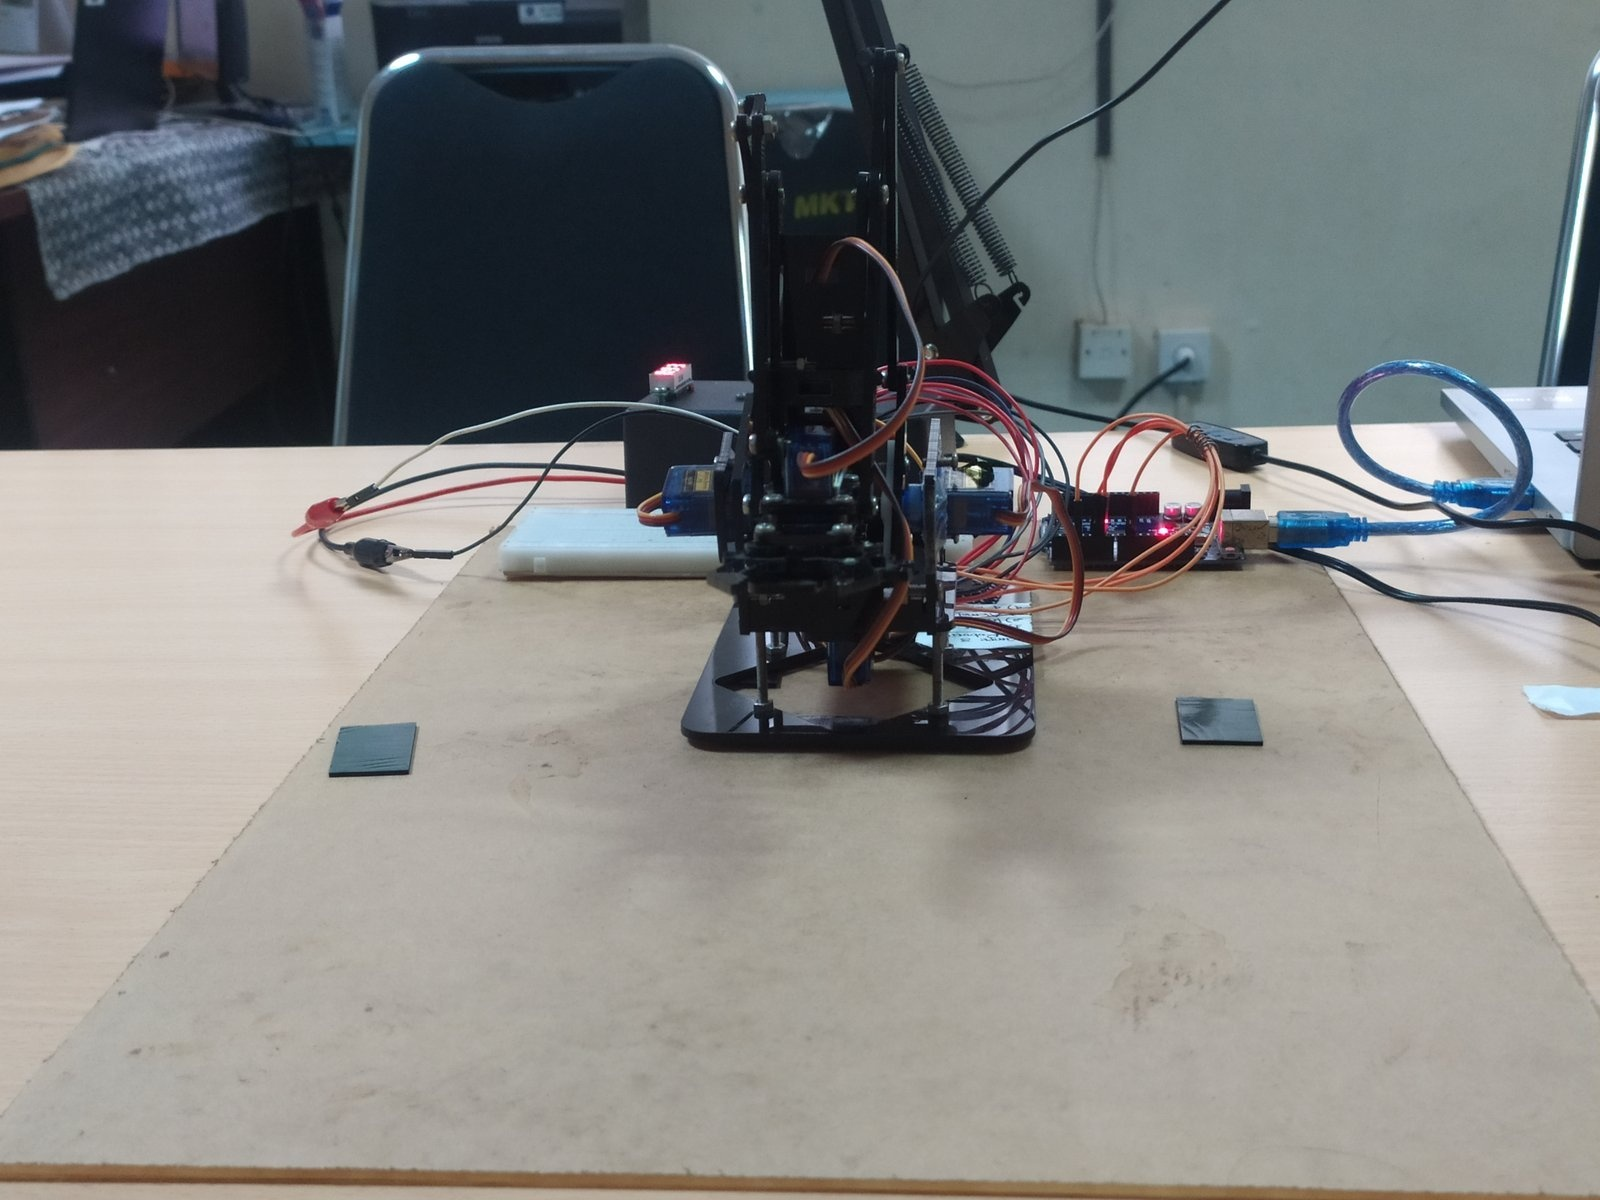
\includegraphics[width=\textwidth]{Gambar/Gambar6_4_mearm_sudut_depan_alternatif.jpg}
        \caption{meArm (Sudut Alternatif)}
        \label{fig:app_6_4}
    \end{subfigure}
    \caption{Dokumentasi Sudut Pandang Lengan meArm}
\end{figure}

\begin{figure}[htbp]
    \centering
    \begin{subfigure}[b]{0.48\textwidth}
        \centering
        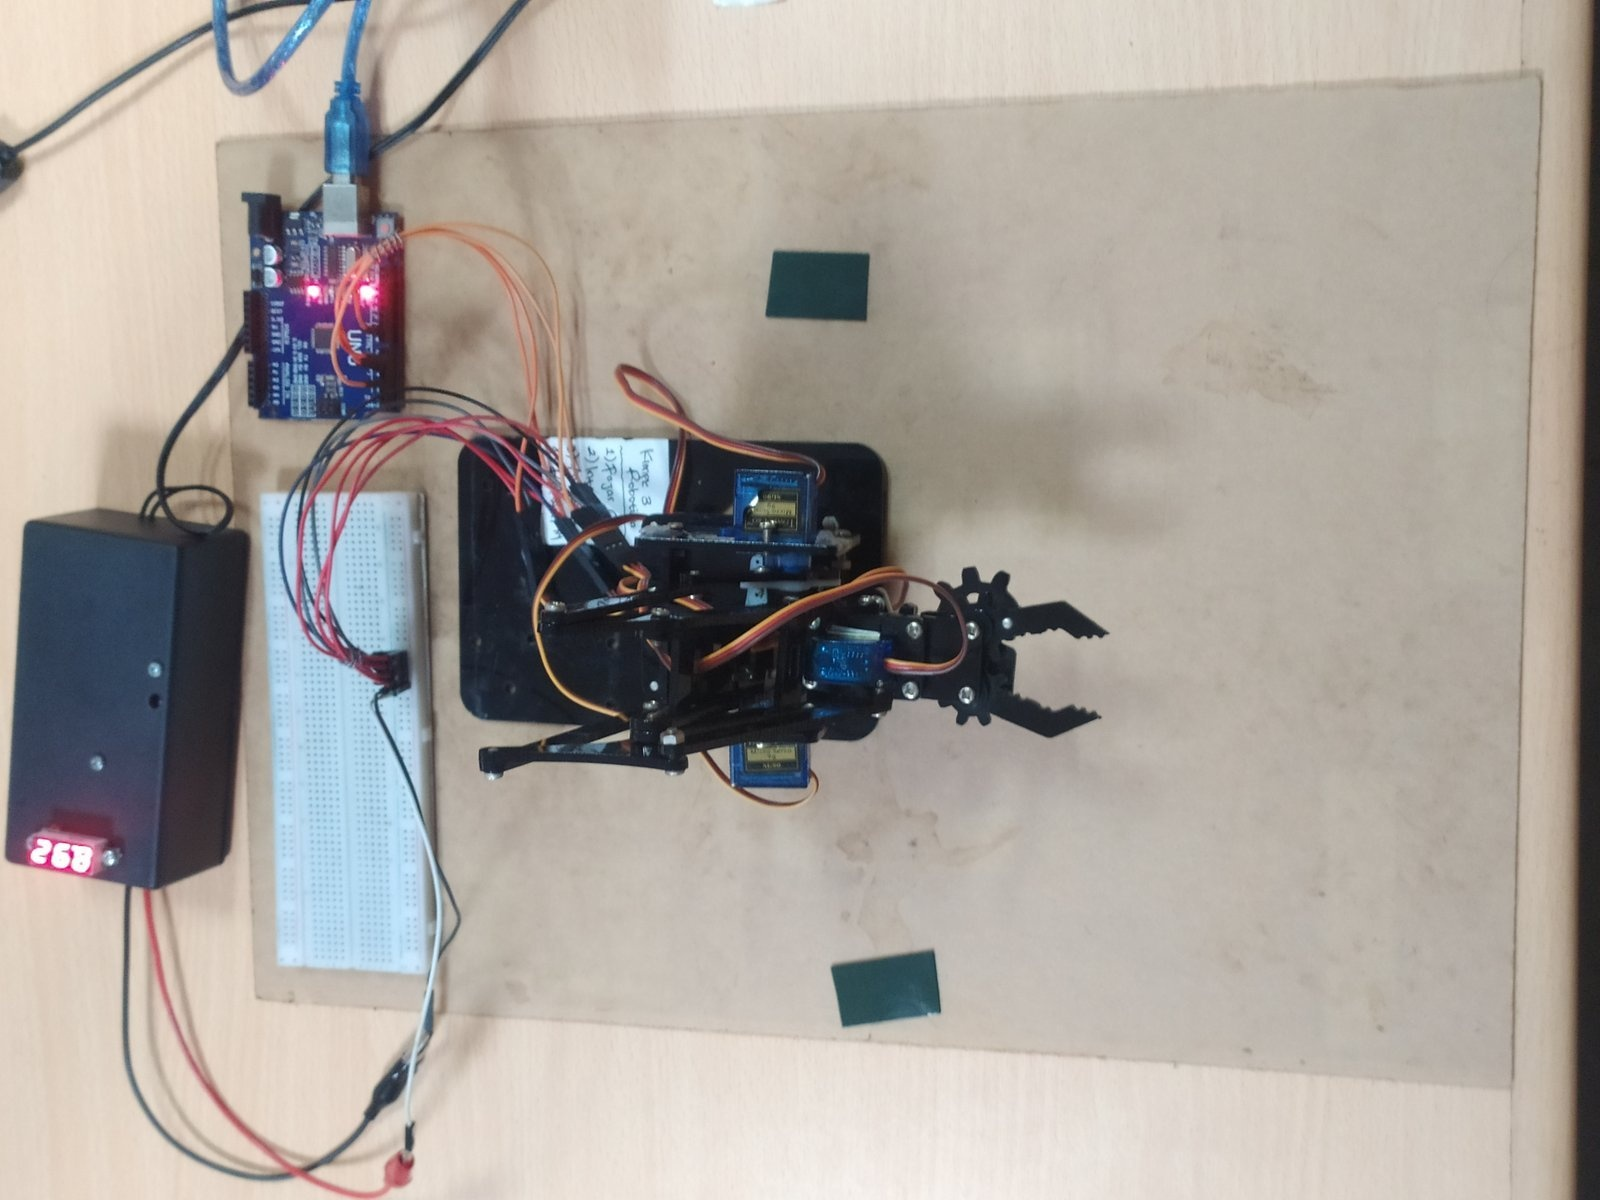
\includegraphics[width=\textwidth]{Gambar/Gambar6_5_perakitan_rangka_akrilik.jpg}
        \caption{Perakitan Rangka Akrilik}
        \label{fig:app_6_5}
    \end{subfigure}
    \hfill
    \begin{subfigure}[b]{0.48\textwidth}
        \centering
        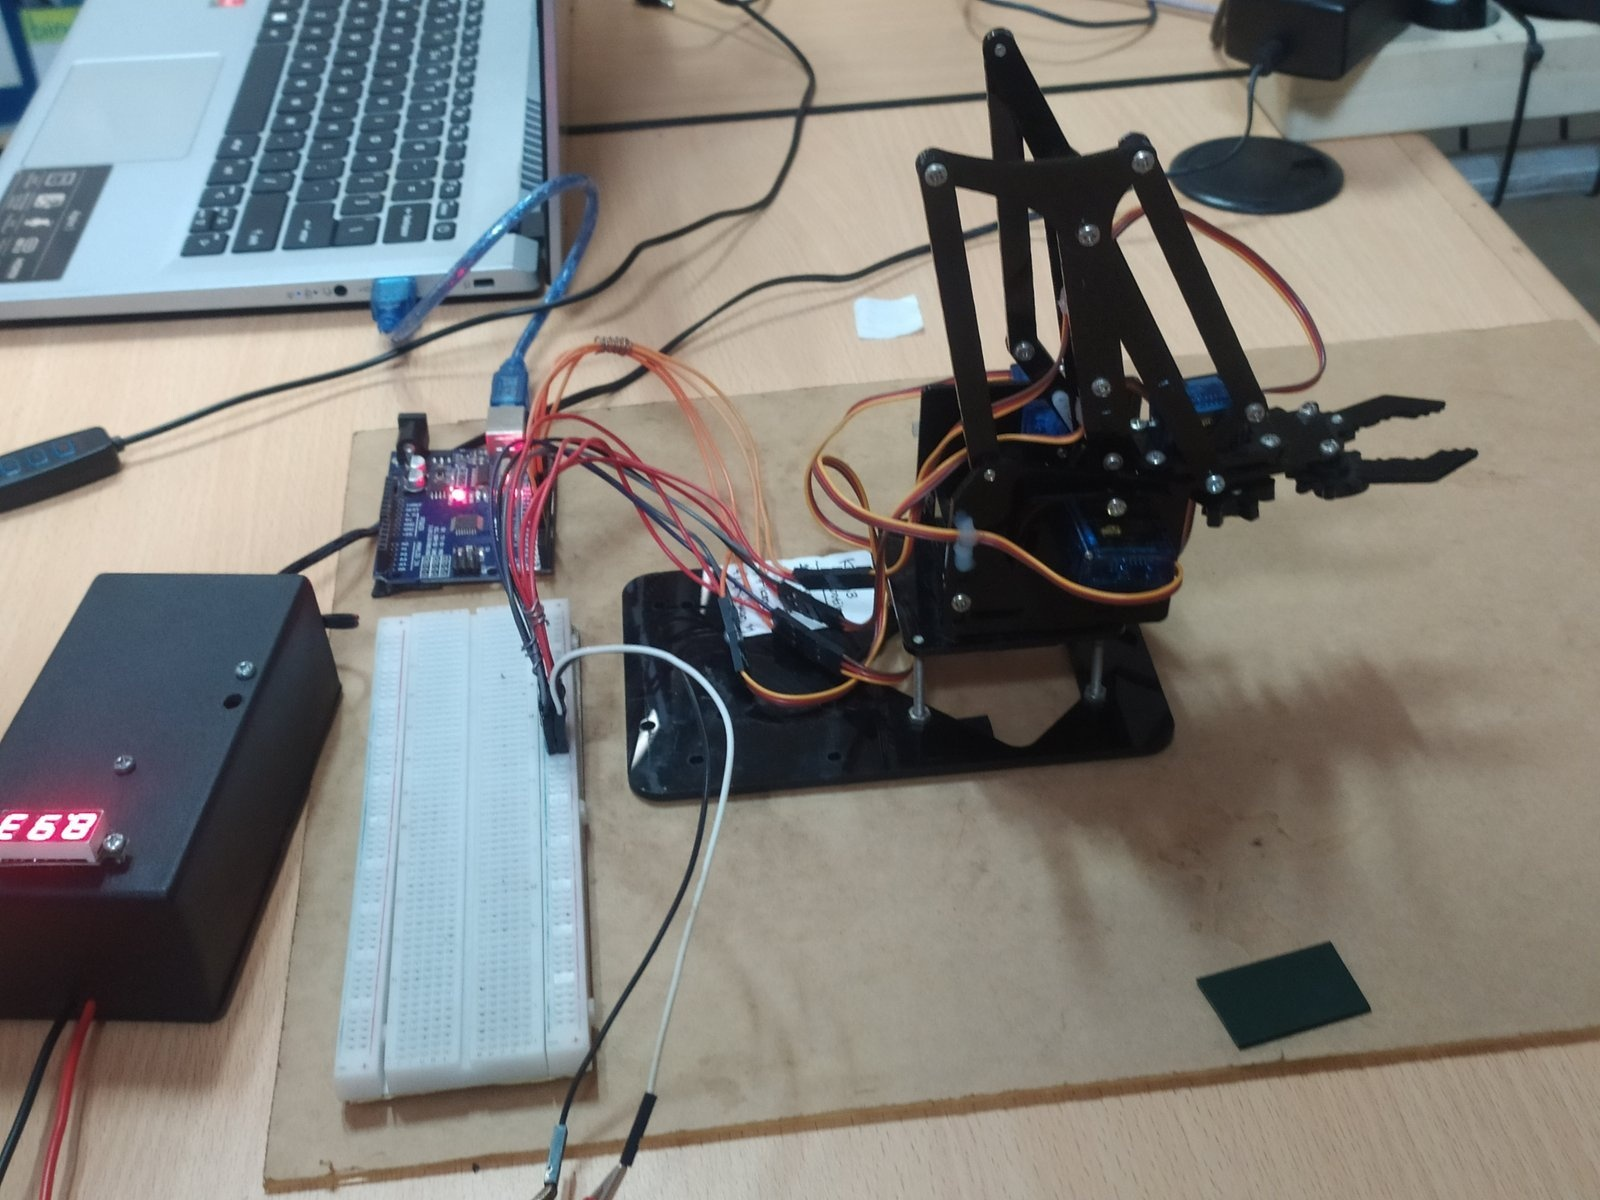
\includegraphics[width=\textwidth]{Gambar/Gambar6_6_penataan_pengkabelan_servo.jpg}
        \caption{Penataan Pengkabelan Servo}
        \label{fig:app_6_6}
    \end{subfigure}
    \caption{Proses Perakitan dan Pengkabelan meArm}
\end{figure}

\begin{figure}[htbp]
    \centering
    \begin{subfigure}[b]{0.48\textwidth}
        \centering
        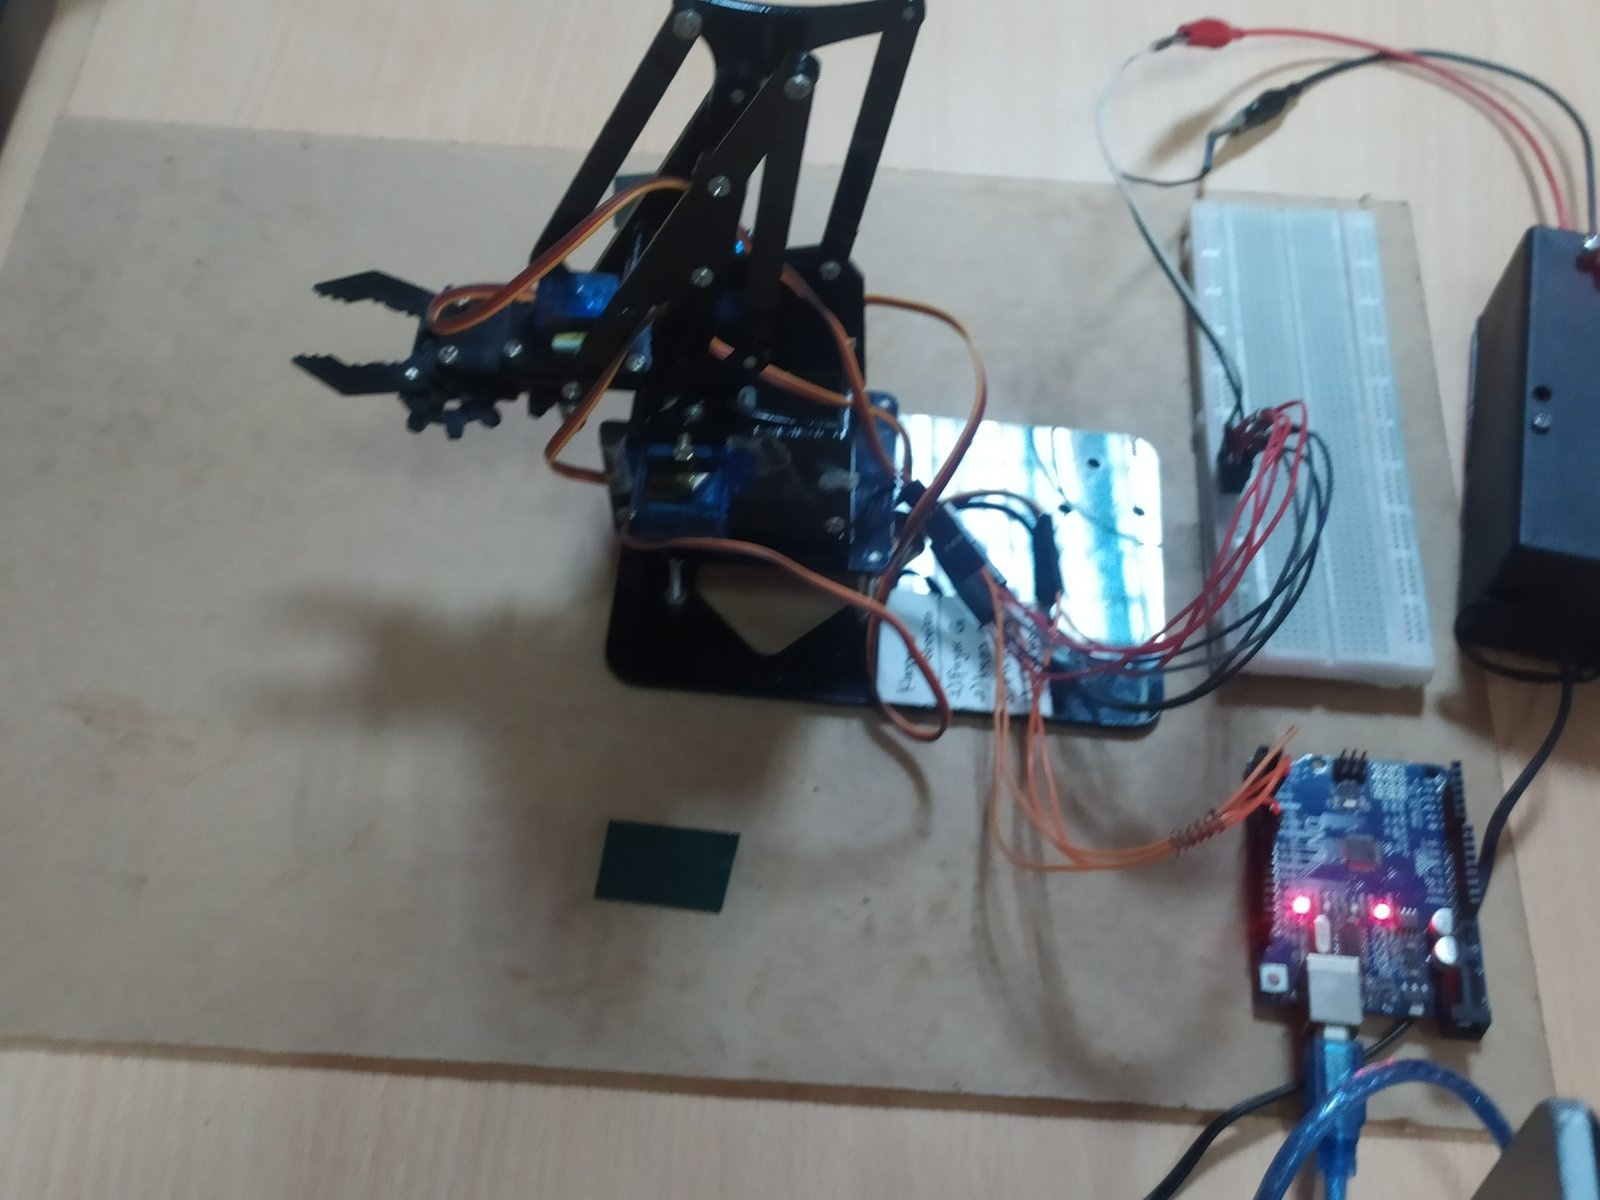
\includegraphics[width=\textwidth]{Gambar/Gambar6_7_detail_sambungan_tautan.jpg}
        \caption{Detail Sambungan Tautan Mekanika}
        \label{fig:app_6_7}
    \end{subfigure}
    \hfill
    \begin{subfigure}[b]{0.48\textwidth}
        \centering
        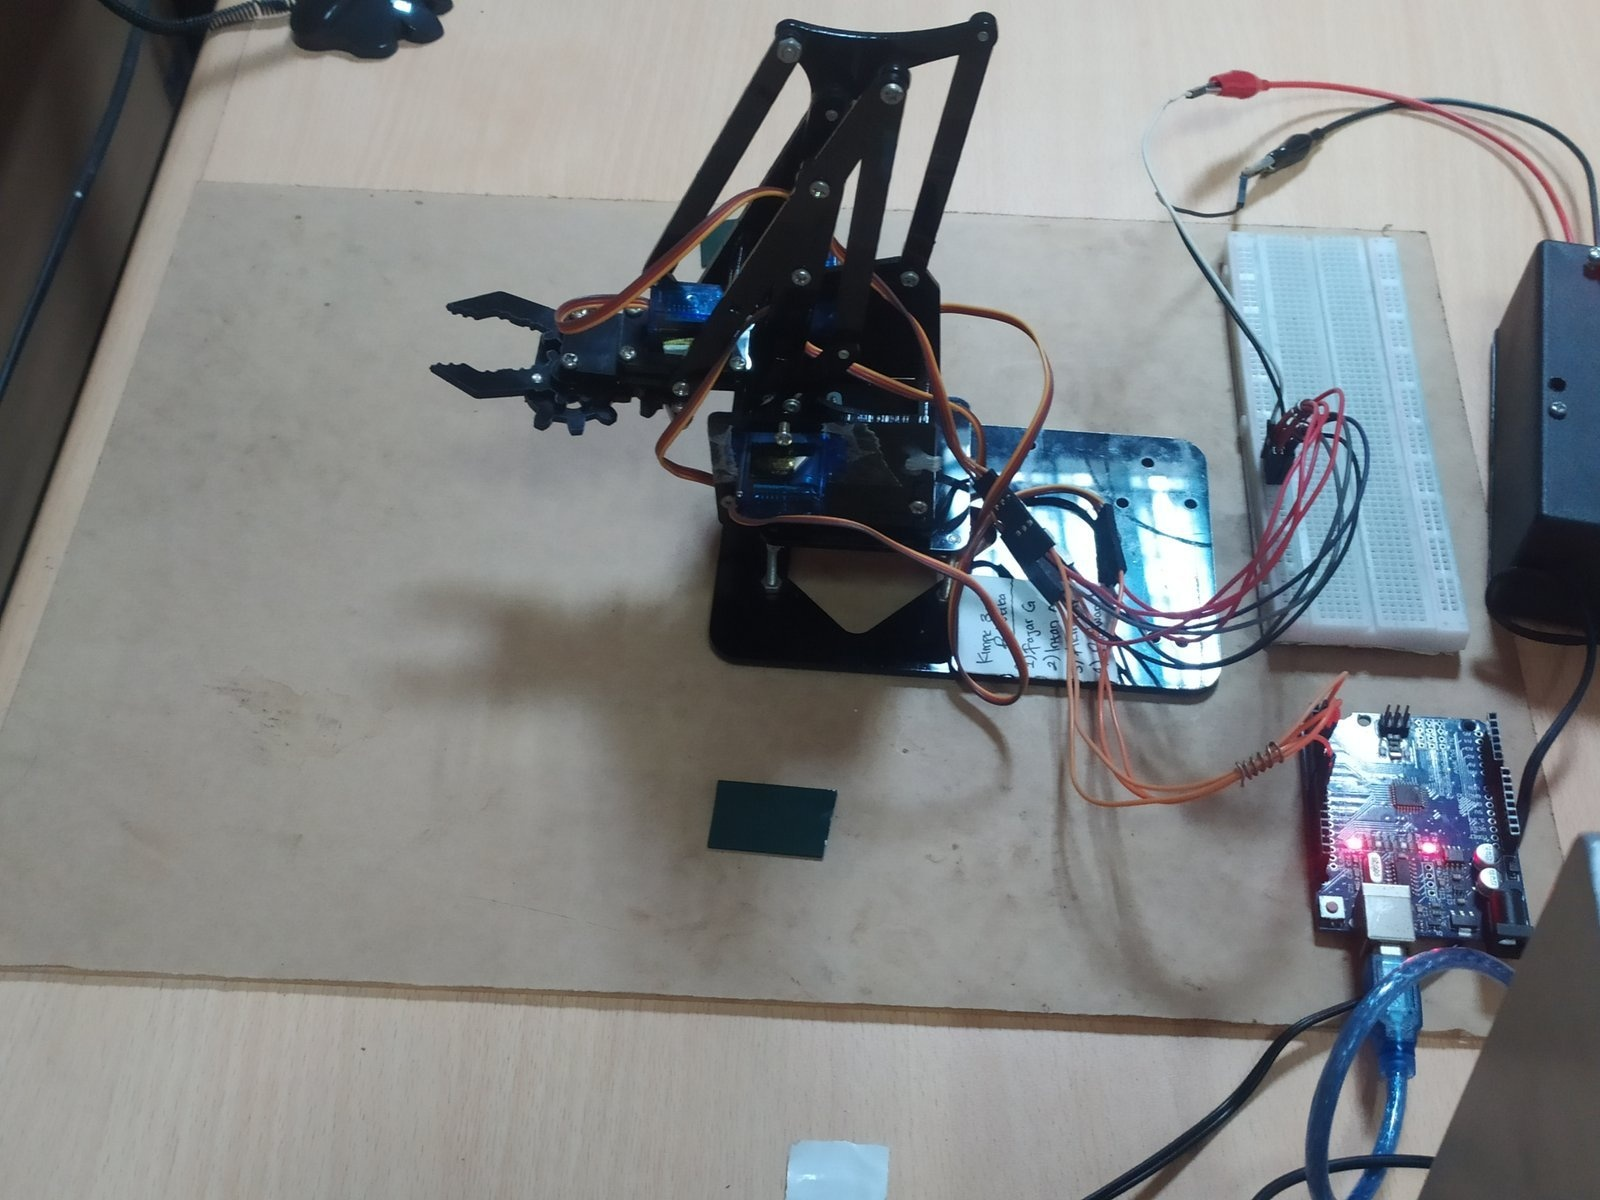
\includegraphics[width=\textwidth]{Gambar/Gambar6_8_pengujian_fleksibilitas_sendi.jpg}
        \caption{Pengujian Fleksibilitas Sendi}
        \label{fig:app_6_8}
    \end{subfigure}
    \caption{Pemeriksaan Mekanika Sambungan meArm}
\end{figure}

\begin{figure}[htbp]
    \centering
    \begin{subfigure}[b]{0.48\textwidth}
        \centering
        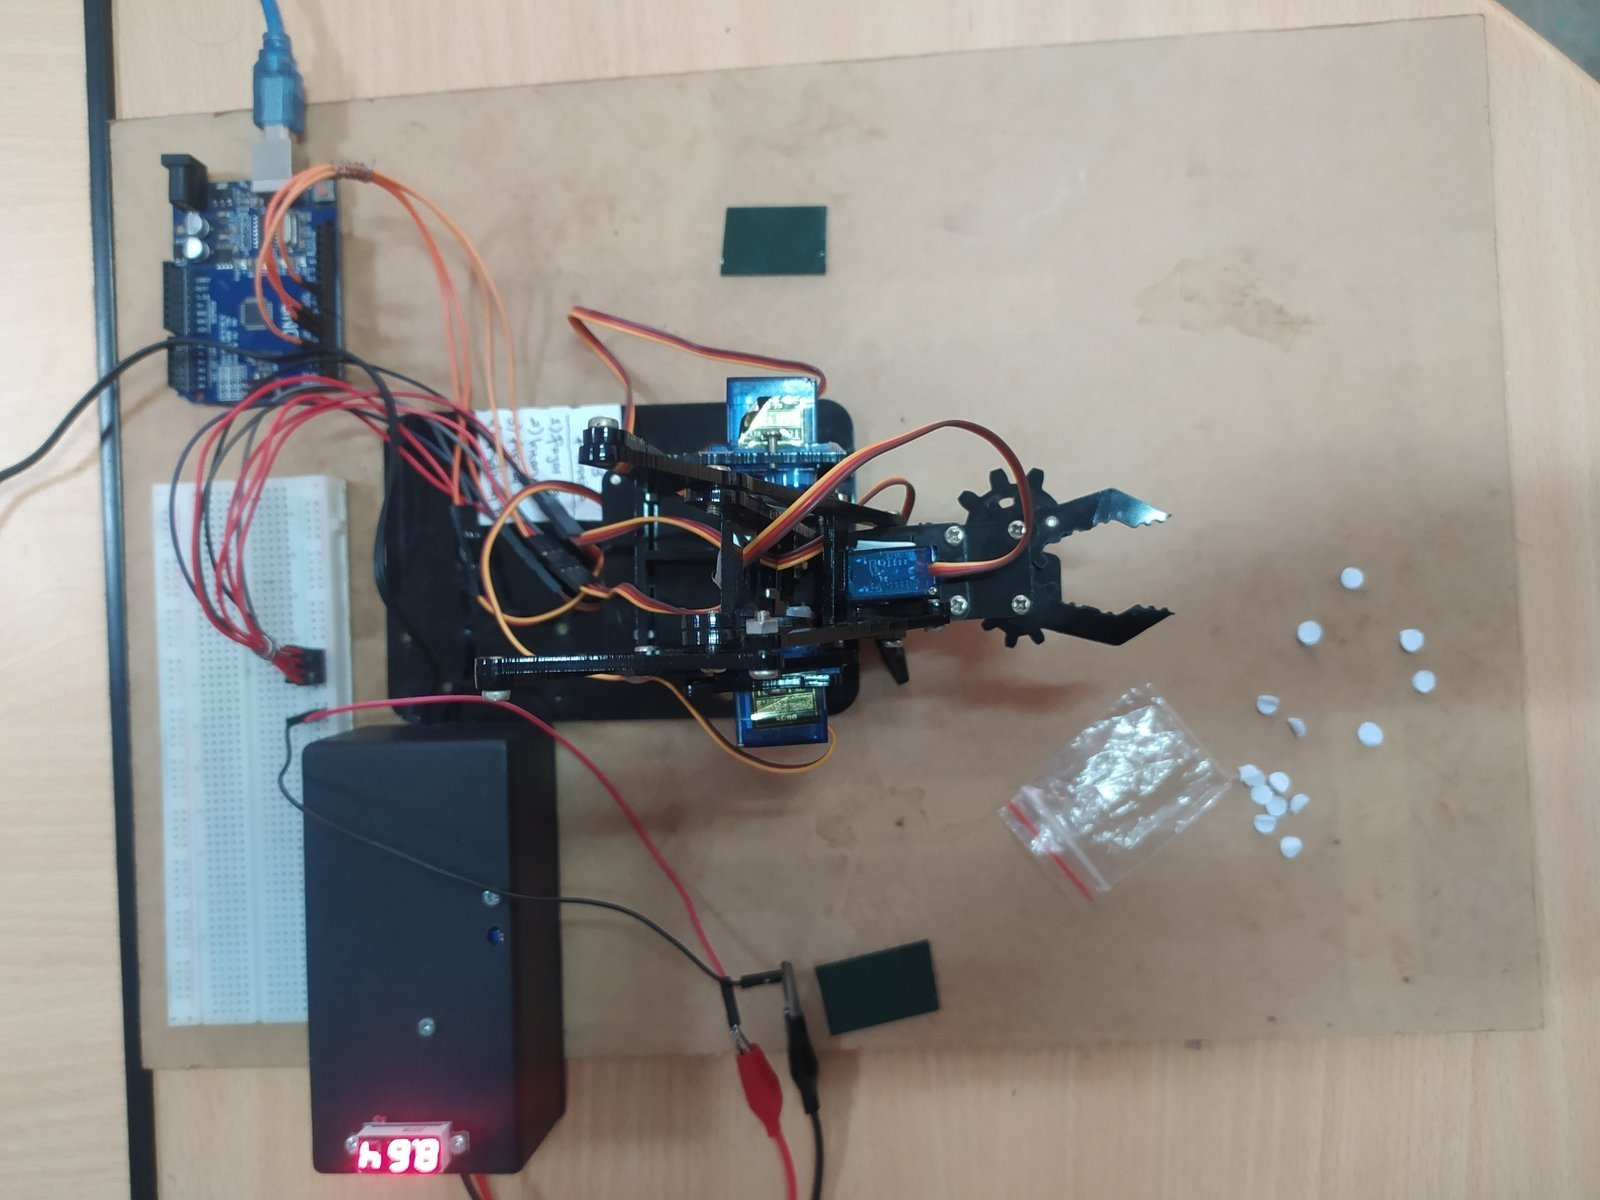
\includegraphics[width=\textwidth]{Gambar/Gambar6_9_integrasi_sistem_mearm.jpg}
        \caption{Integrasi Sistem di Meja Eksperimen}
        \label{fig:app_6_9}
    \end{subfigure}
    \hfill
    \begin{subfigure}[b]{0.48\textwidth}
        \centering
        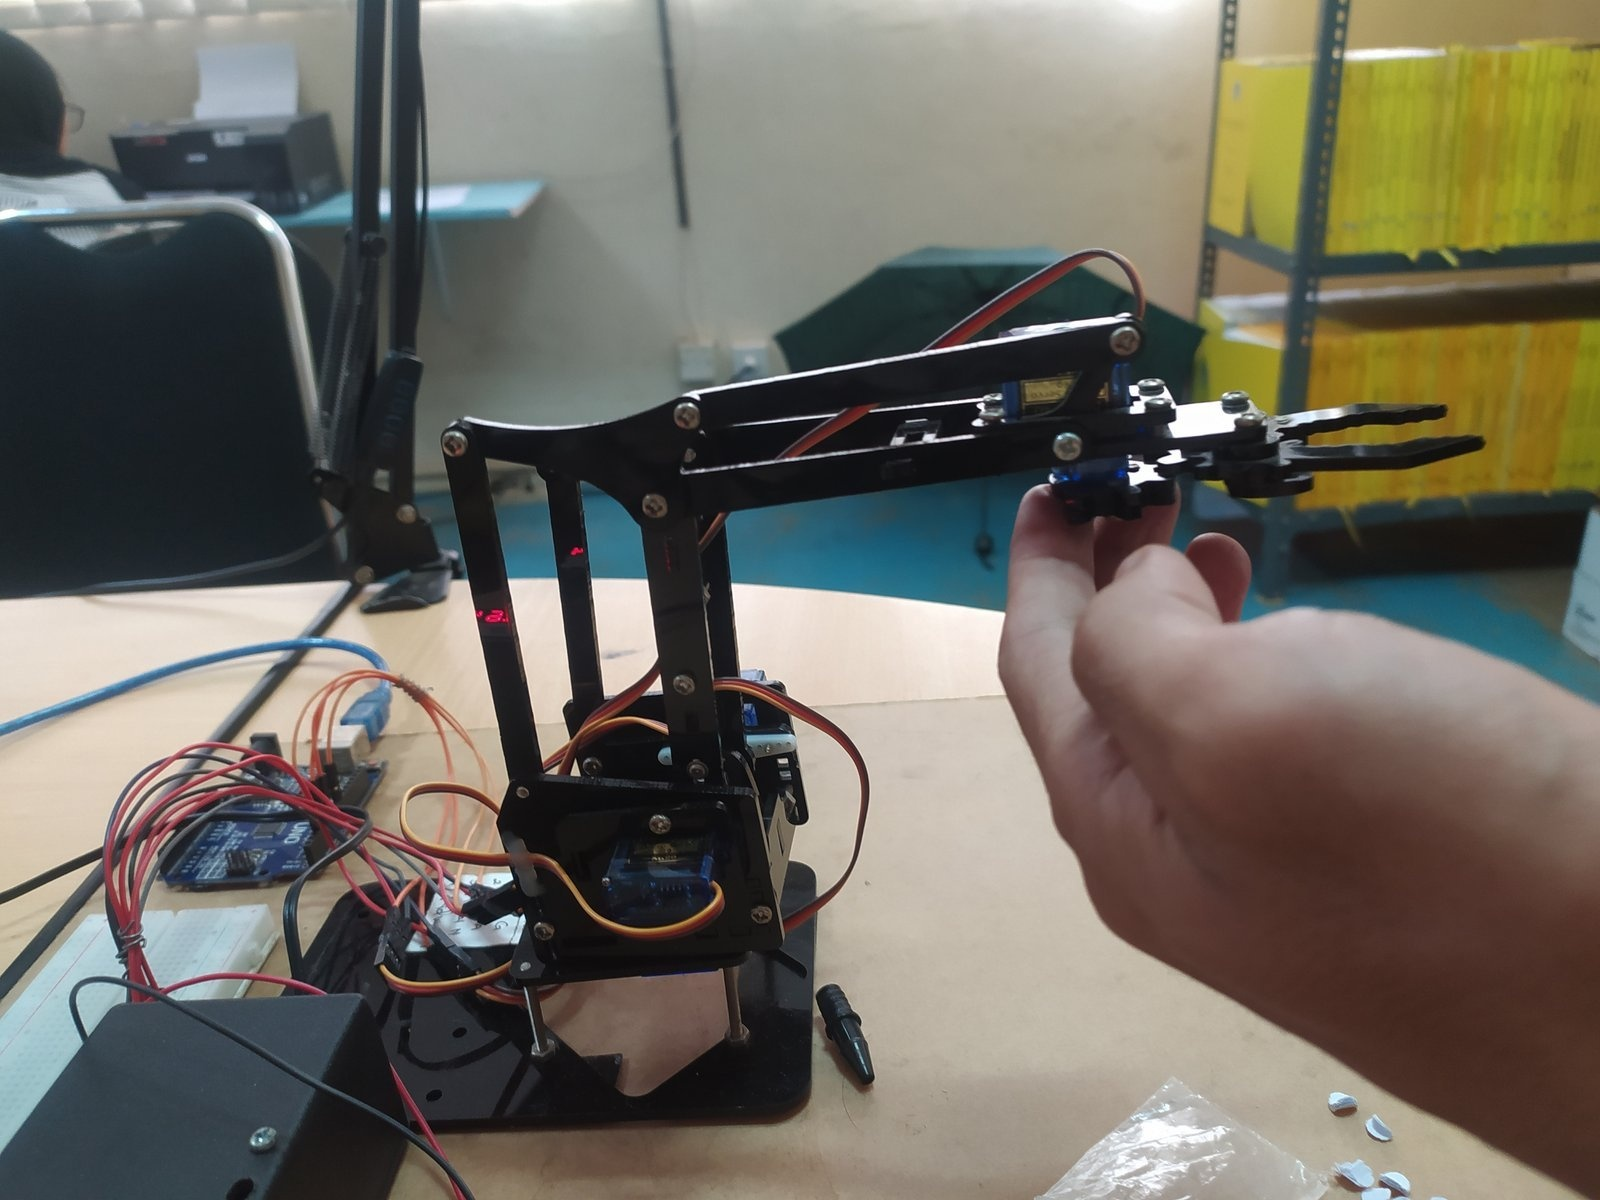
\includegraphics[width=\textwidth]{Gambar/Gambar6_10_pengujian_manuver_ik_sesi1.jpg}
        \caption{Uji Manuver Kinematika Balikan Sesi 1}
        \label{fig:app_6_10}
    \end{subfigure}
    \caption{Pengujian Eksperimental meArm}
\end{figure}

\begin{figure}[htbp]
    \centering
    \begin{subfigure}[b]{0.48\textwidth}
        \centering
        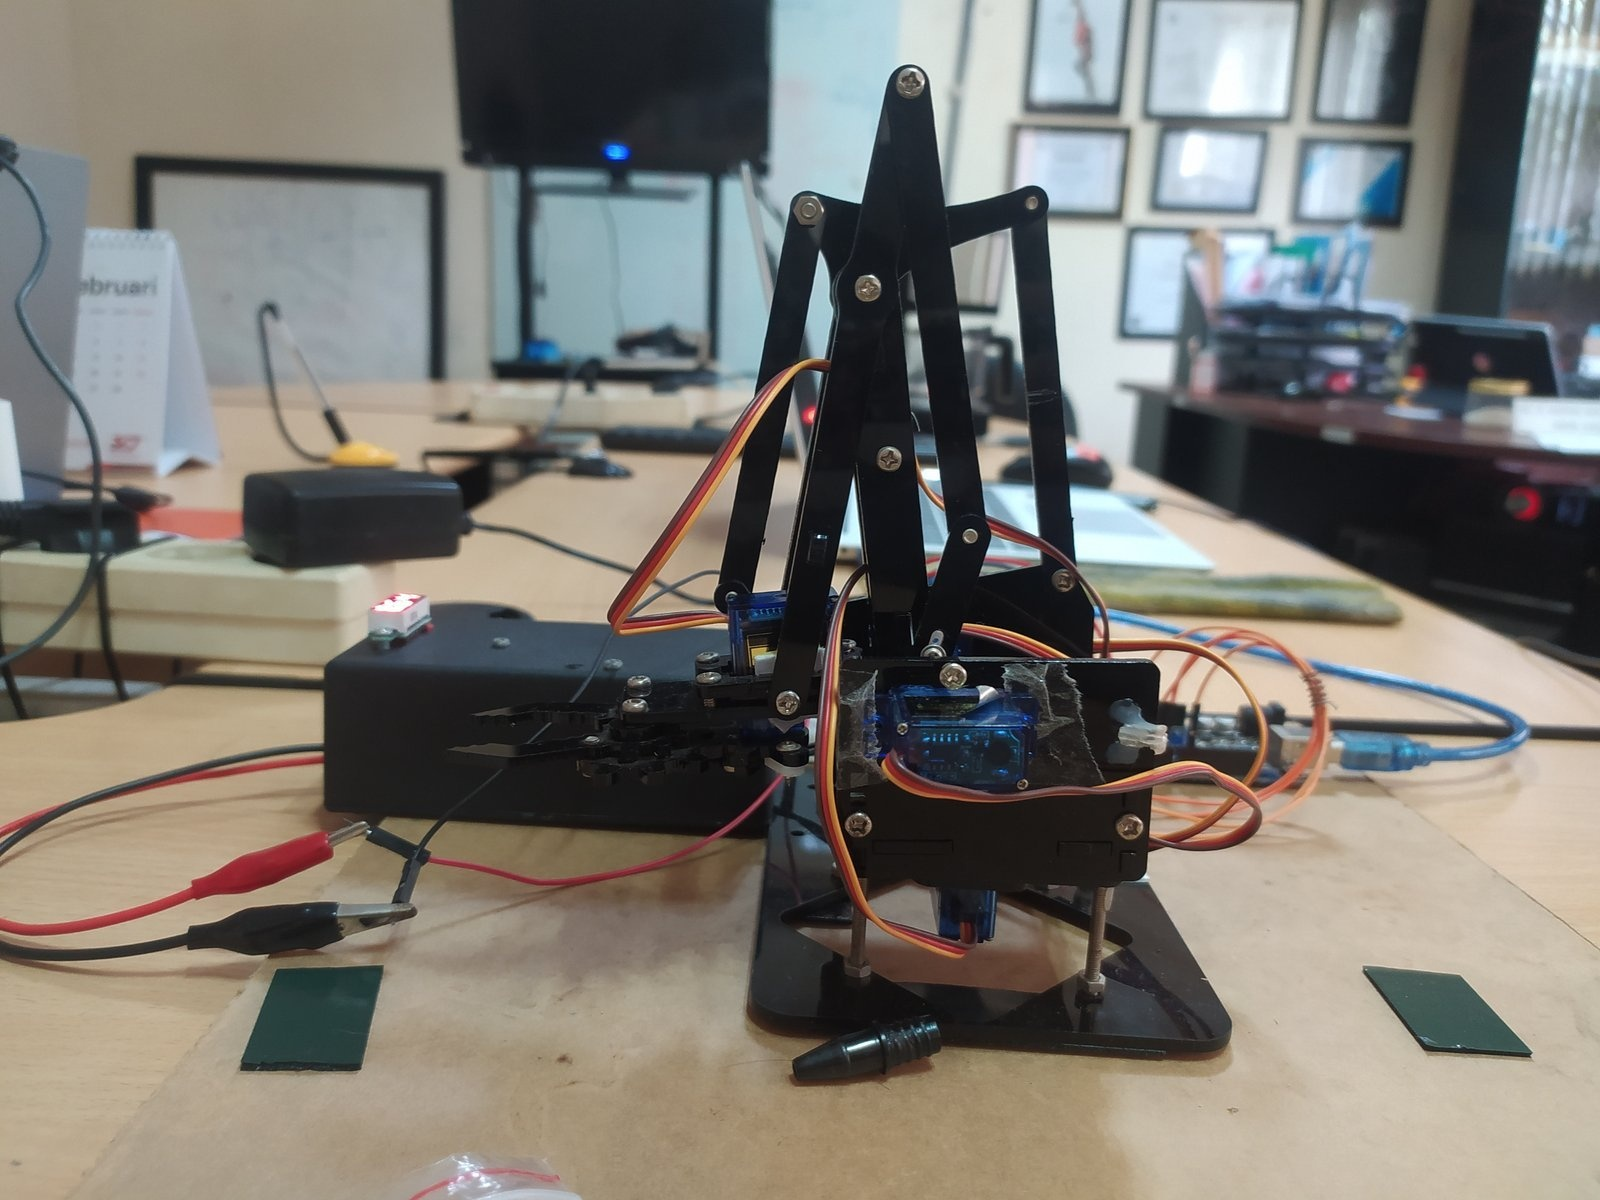
\includegraphics[width=\textwidth]{Gambar/Gambar6_11_pengujian_manuver_ik_sesi2.jpg}
        \caption{Uji Manuver Kinematika Balikan Sesi 2}
        \label{fig:app_6_11}
    \end{subfigure}
    \hfill
    \begin{subfigure}[b]{0.48\textwidth}
        \centering
        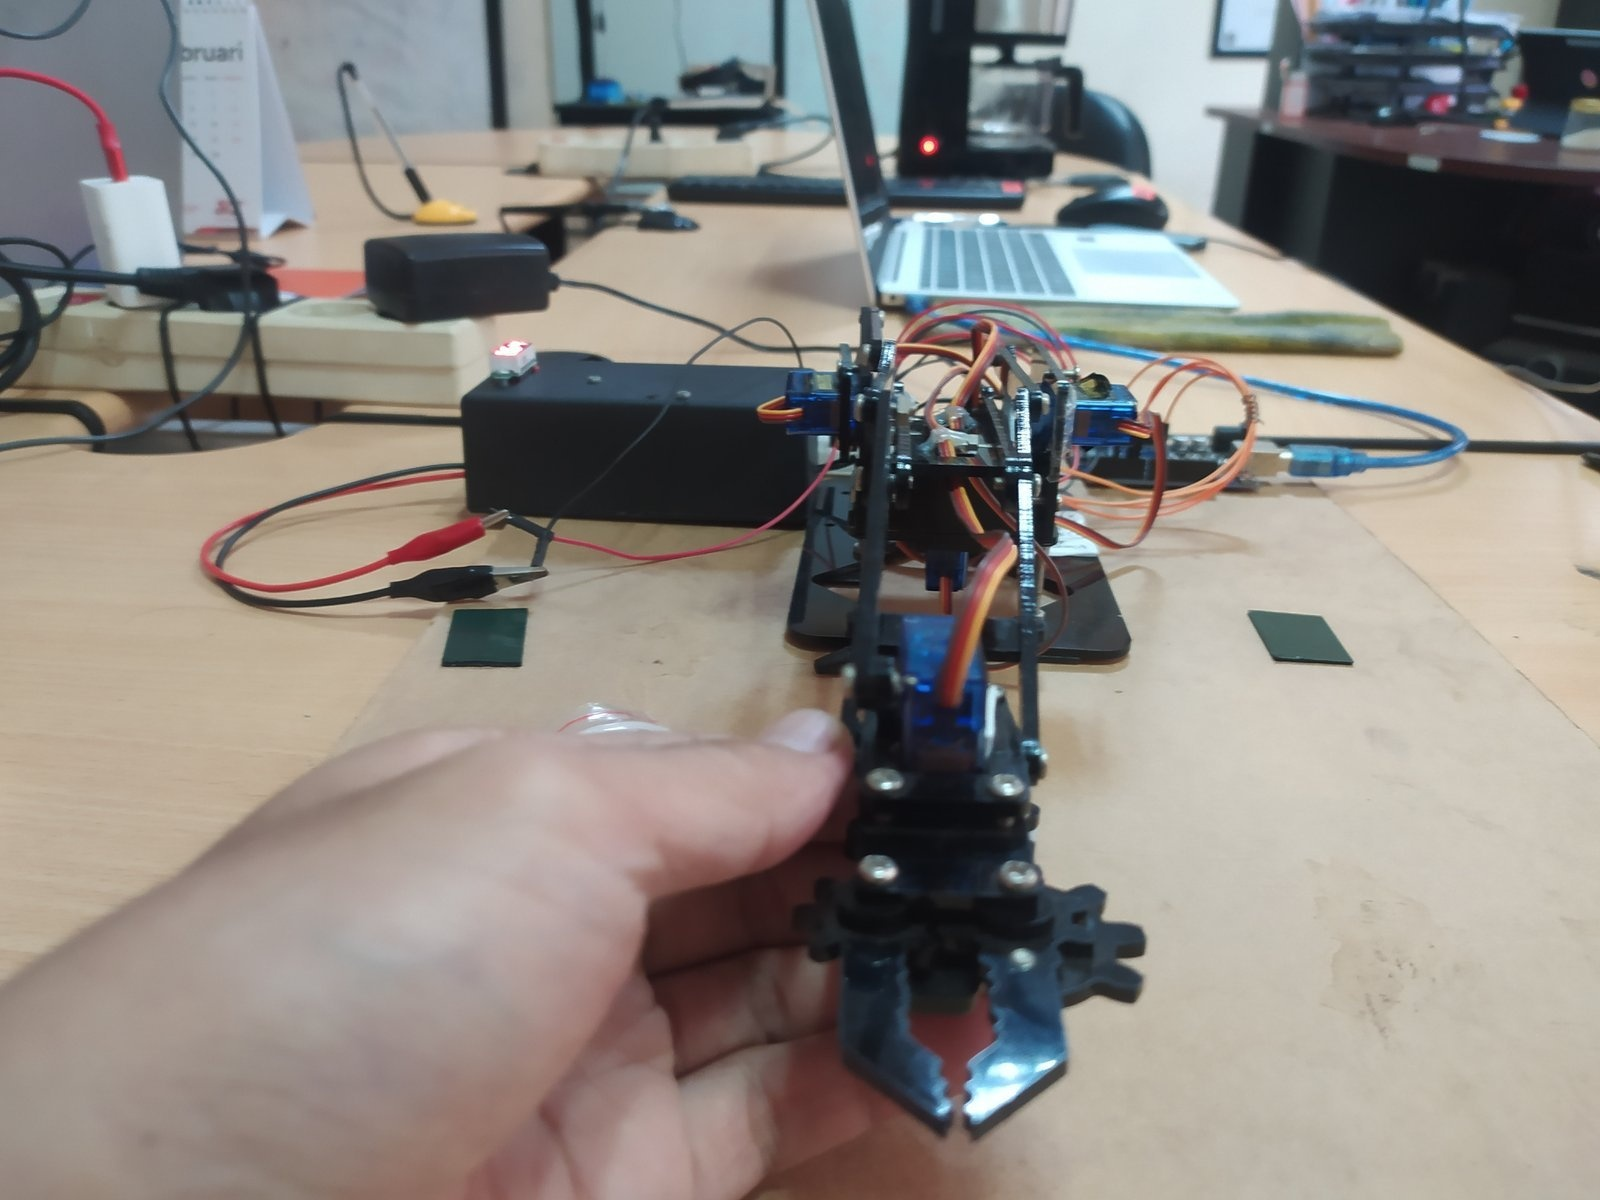
\includegraphics[width=\textwidth]{Gambar/Gambar6_12_pengujian_jangkauan_capit.jpg}
        \caption{Pengujian Jangkauan dan Capit}
        \label{fig:app_6_12}
    \end{subfigure}
    \caption{Pengujian Jangkauan Kerja dan Capit meArm}
\end{figure}

\begin{figure}[htbp]
    \centering
    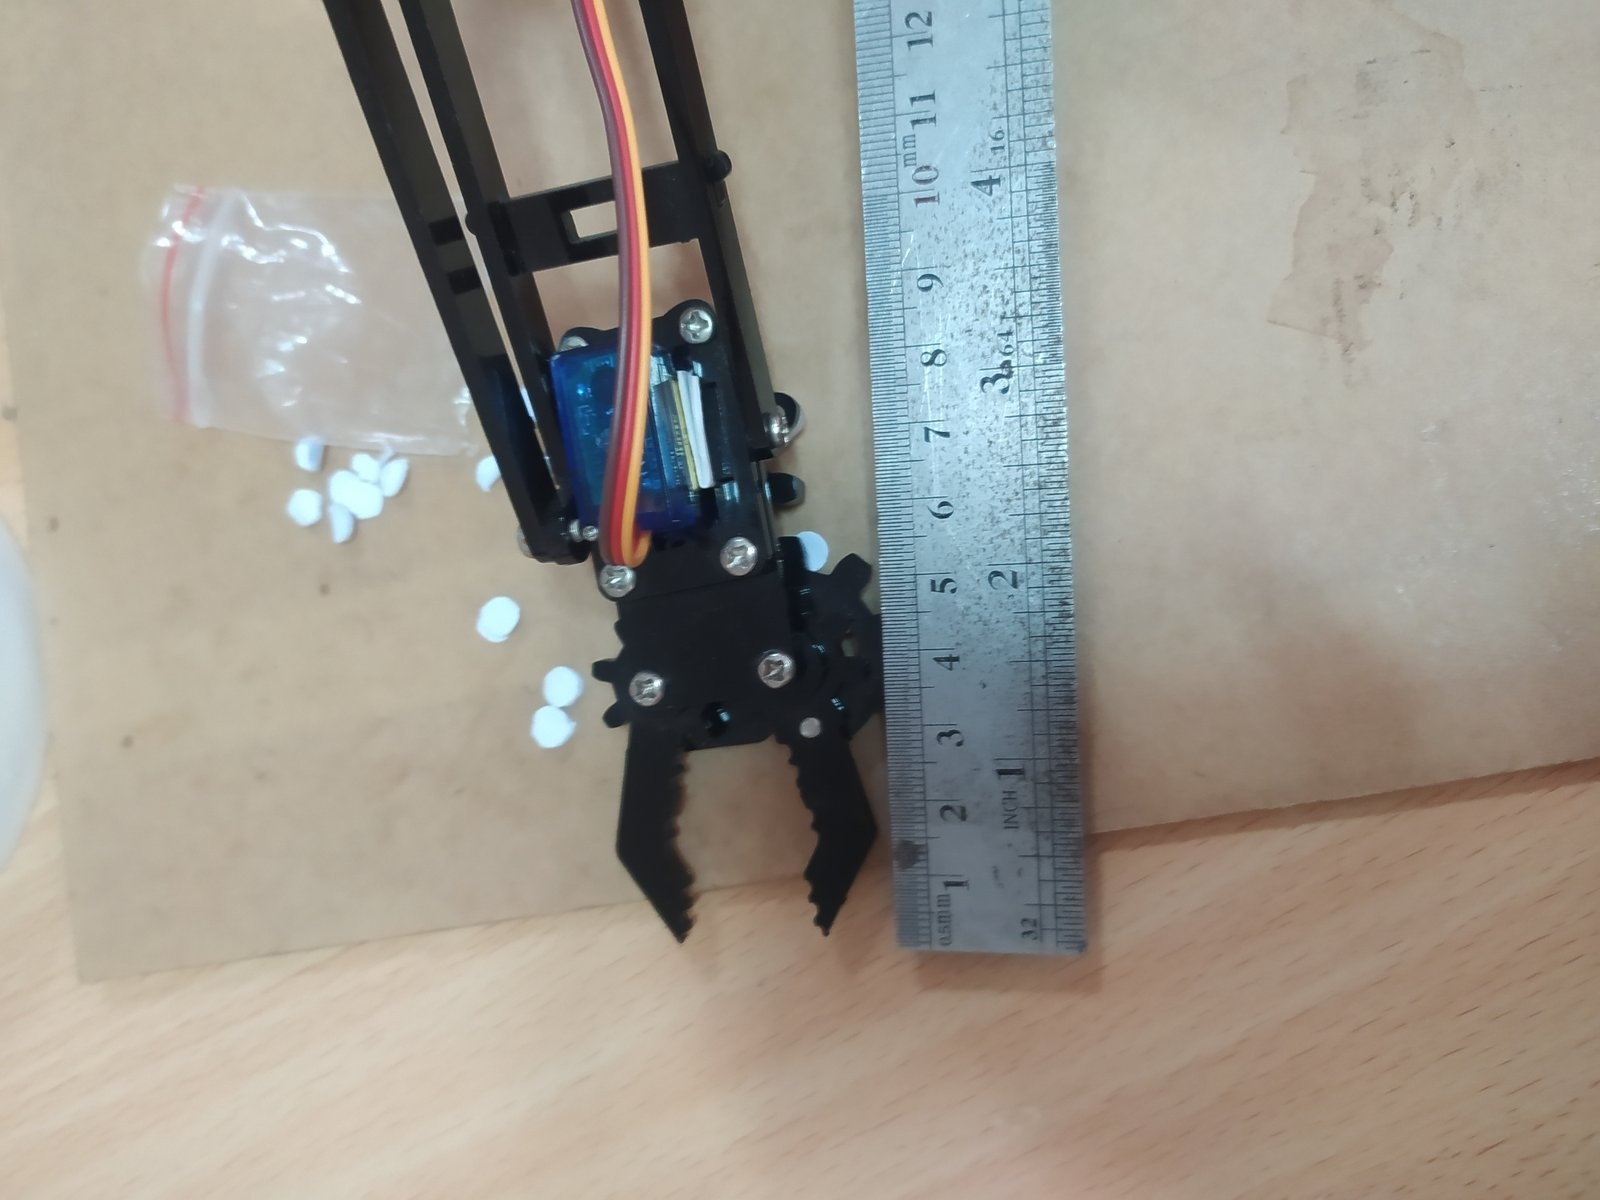
\includegraphics[width=0.75\textwidth]{Gambar/Gambar6_13_pengujian_respons_gerak_sibi.jpg}
    \caption{Pengujian Respons Gerak meArm Berbasis Isyarat SIBI}
    \label{fig:app_6_13}
\end{figure}

\newpage
\subsection*{4.2 Dokumentasi Perangkat dan Teleoperasi Dobot Magician}

\begin{figure}[htbp]
    \centering
    \begin{subfigure}[b]{0.48\textwidth}
        \centering
        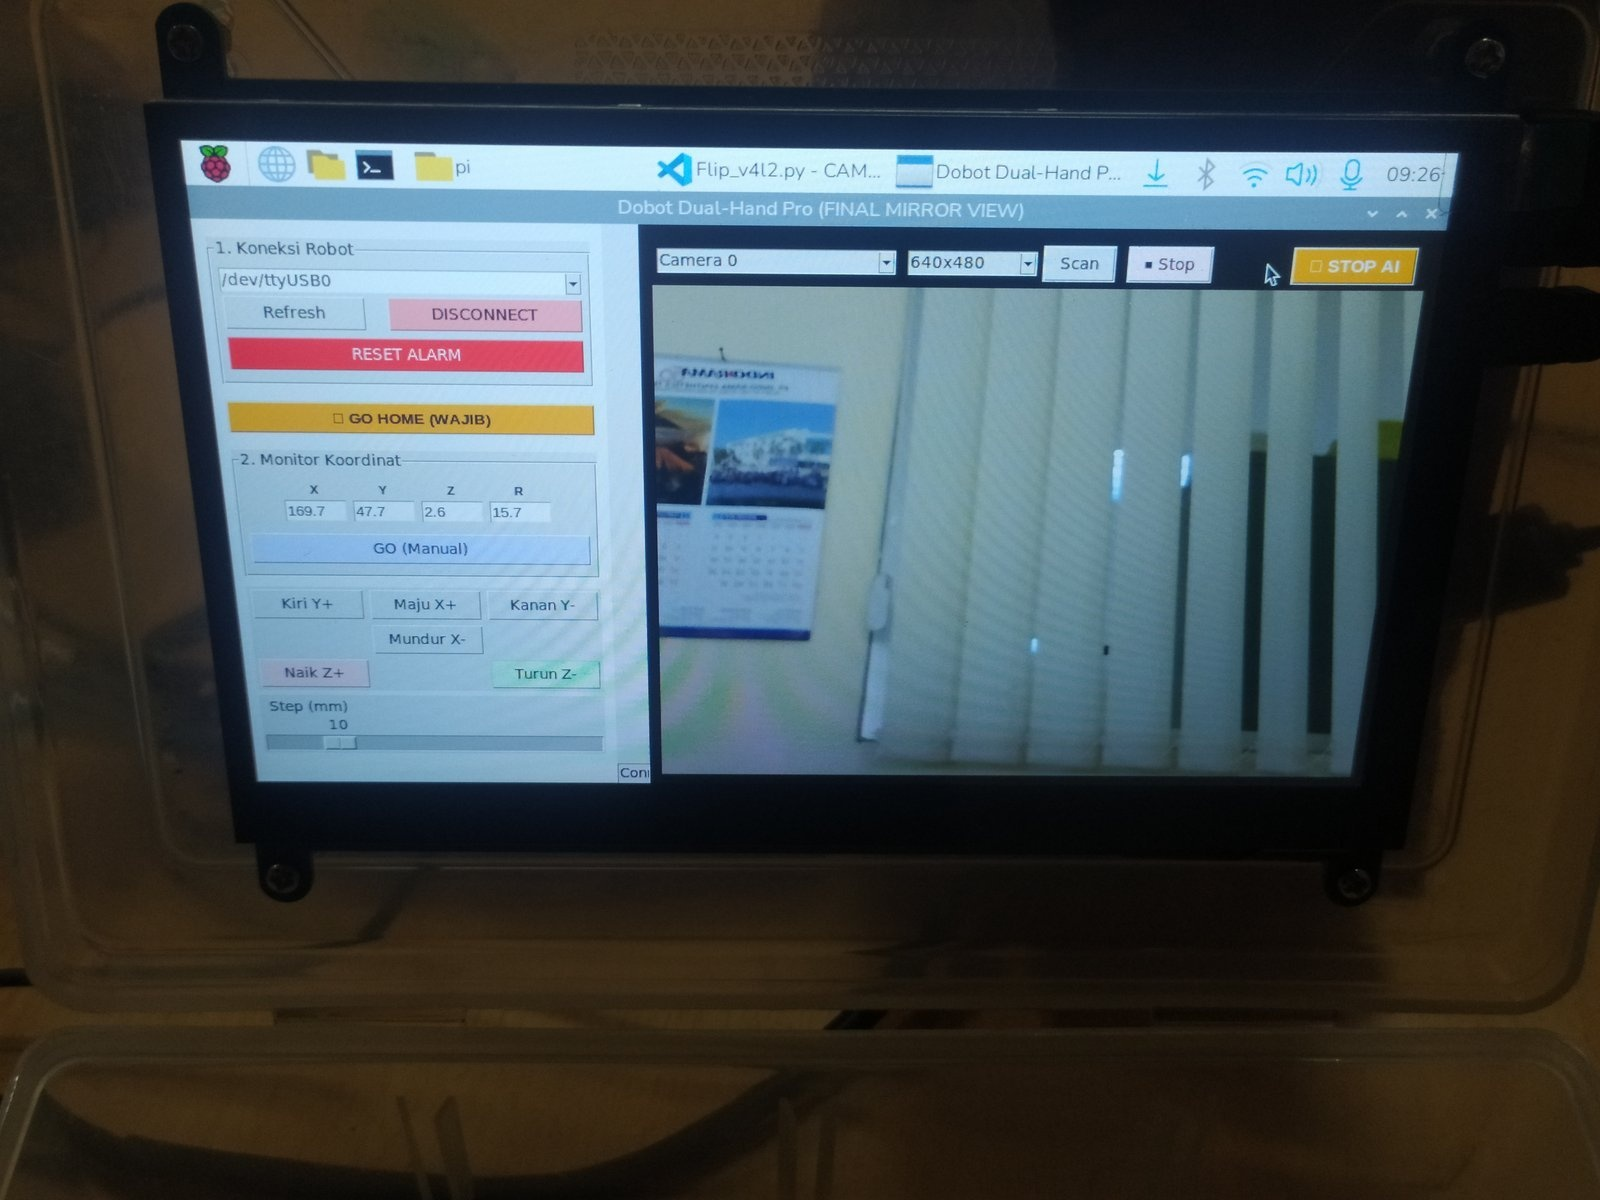
\includegraphics[width=\textwidth]{Gambar/Gambar6_14_antarmuka_pelacakan_dobot.jpg}
        \caption{Antarmuka Pelacakan Tangan}
        \label{fig:app_6_14}
    \end{subfigure}
    \hfill
    \begin{subfigure}[b]{0.48\textwidth}
        \centering
        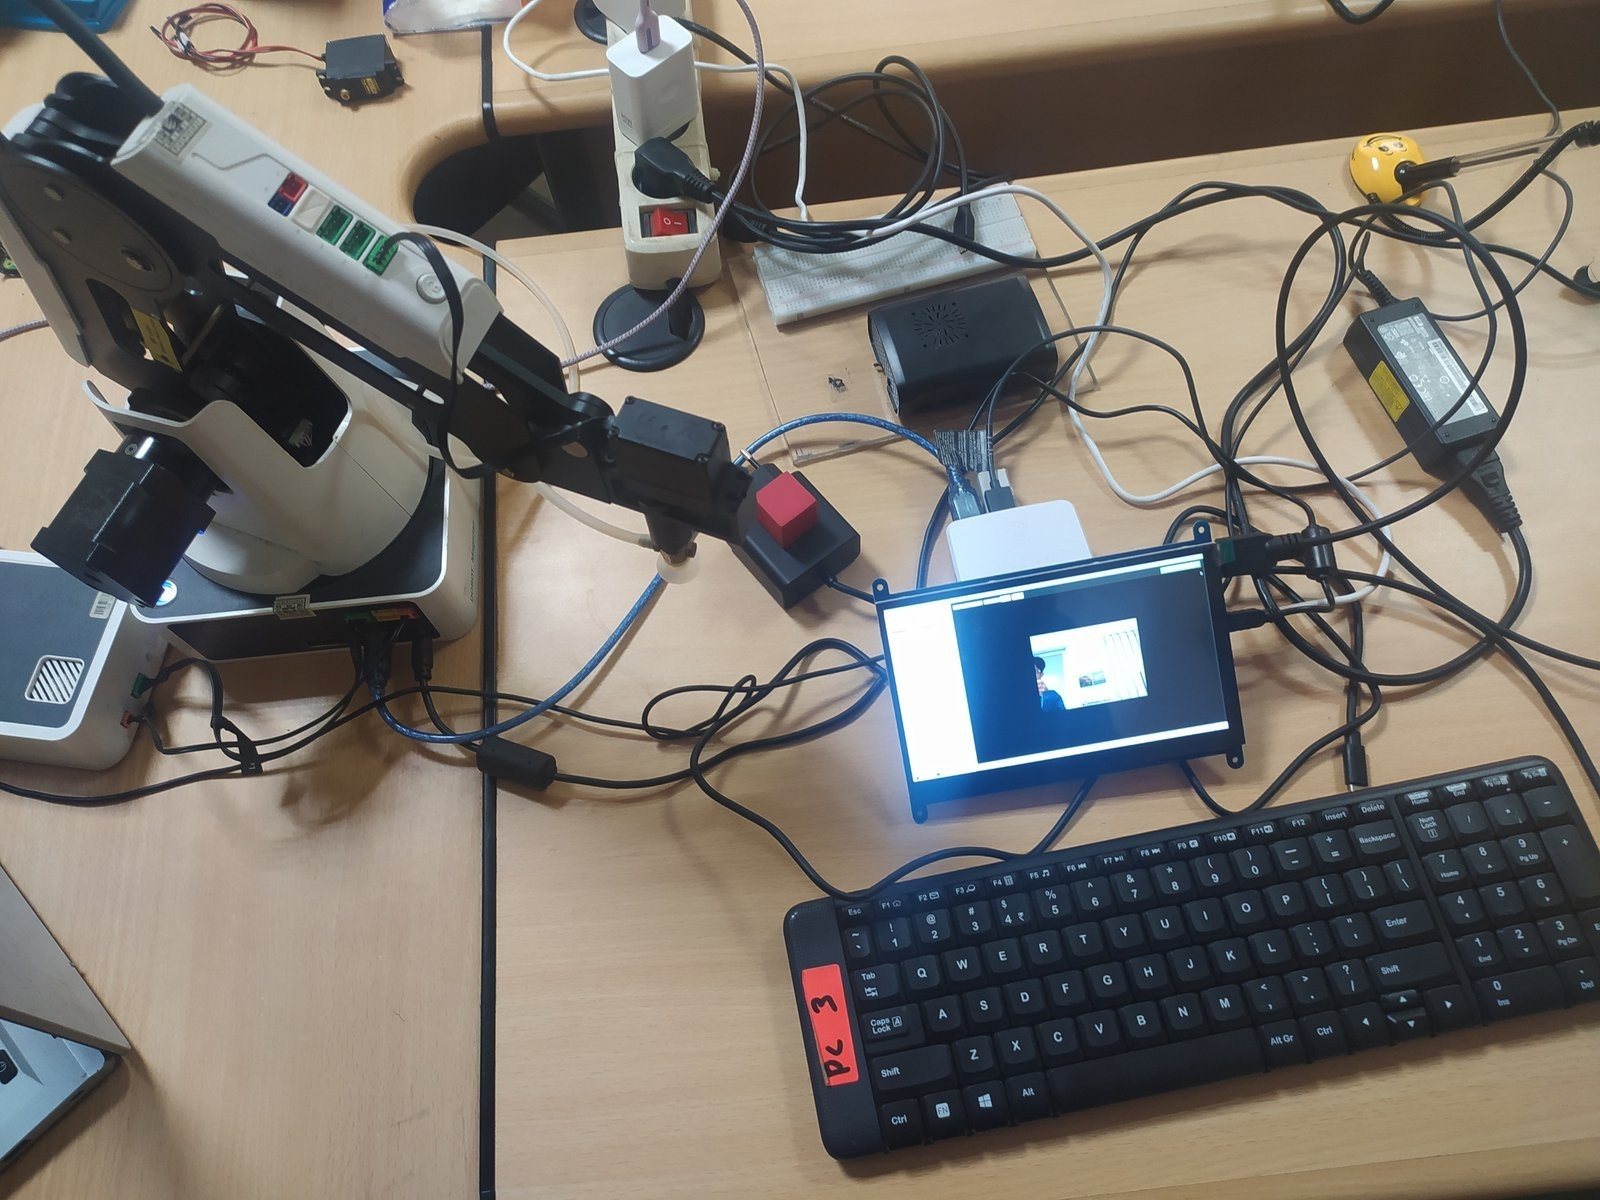
\includegraphics[width=\textwidth]{Gambar/Gambar6_15_stasiun_teleoperasi_dobot1.jpg}
        \caption{Stasiun Kerja Teleoperasi (Sudut 1)}
        \label{fig:app_6_15}
    \end{subfigure}
    \caption{Pengujian Teleoperasi Dobot Magician}
\end{figure}

\begin{figure}[htbp]
    \centering
    \begin{subfigure}[b]{0.48\textwidth}
        \centering
        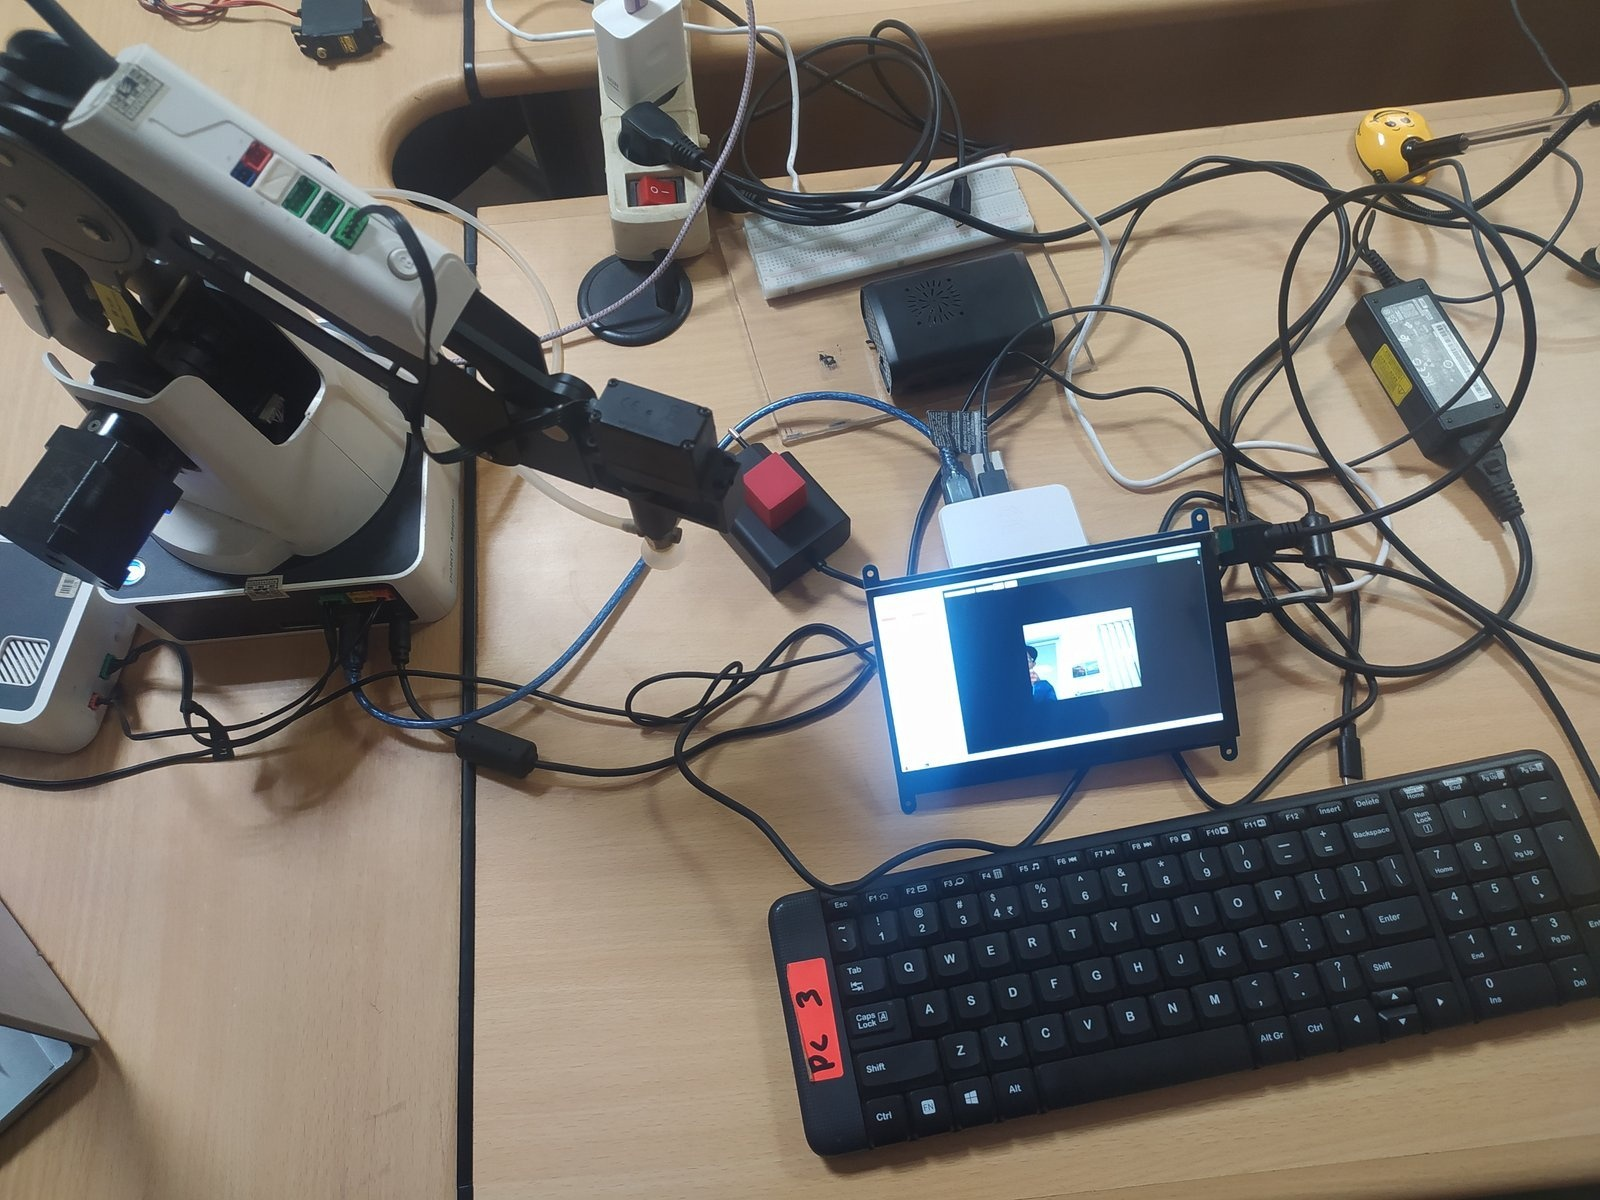
\includegraphics[width=\textwidth]{Gambar/Gambar6_16_stasiun_teleoperasi_dobot2.jpg}
        \caption{Stasiun Kerja Teleoperasi (Sudut 2)}
        \label{fig:app_6_16}
    \end{subfigure}
    \hfill
    \begin{subfigure}[b]{0.48\textwidth}
        \centering
        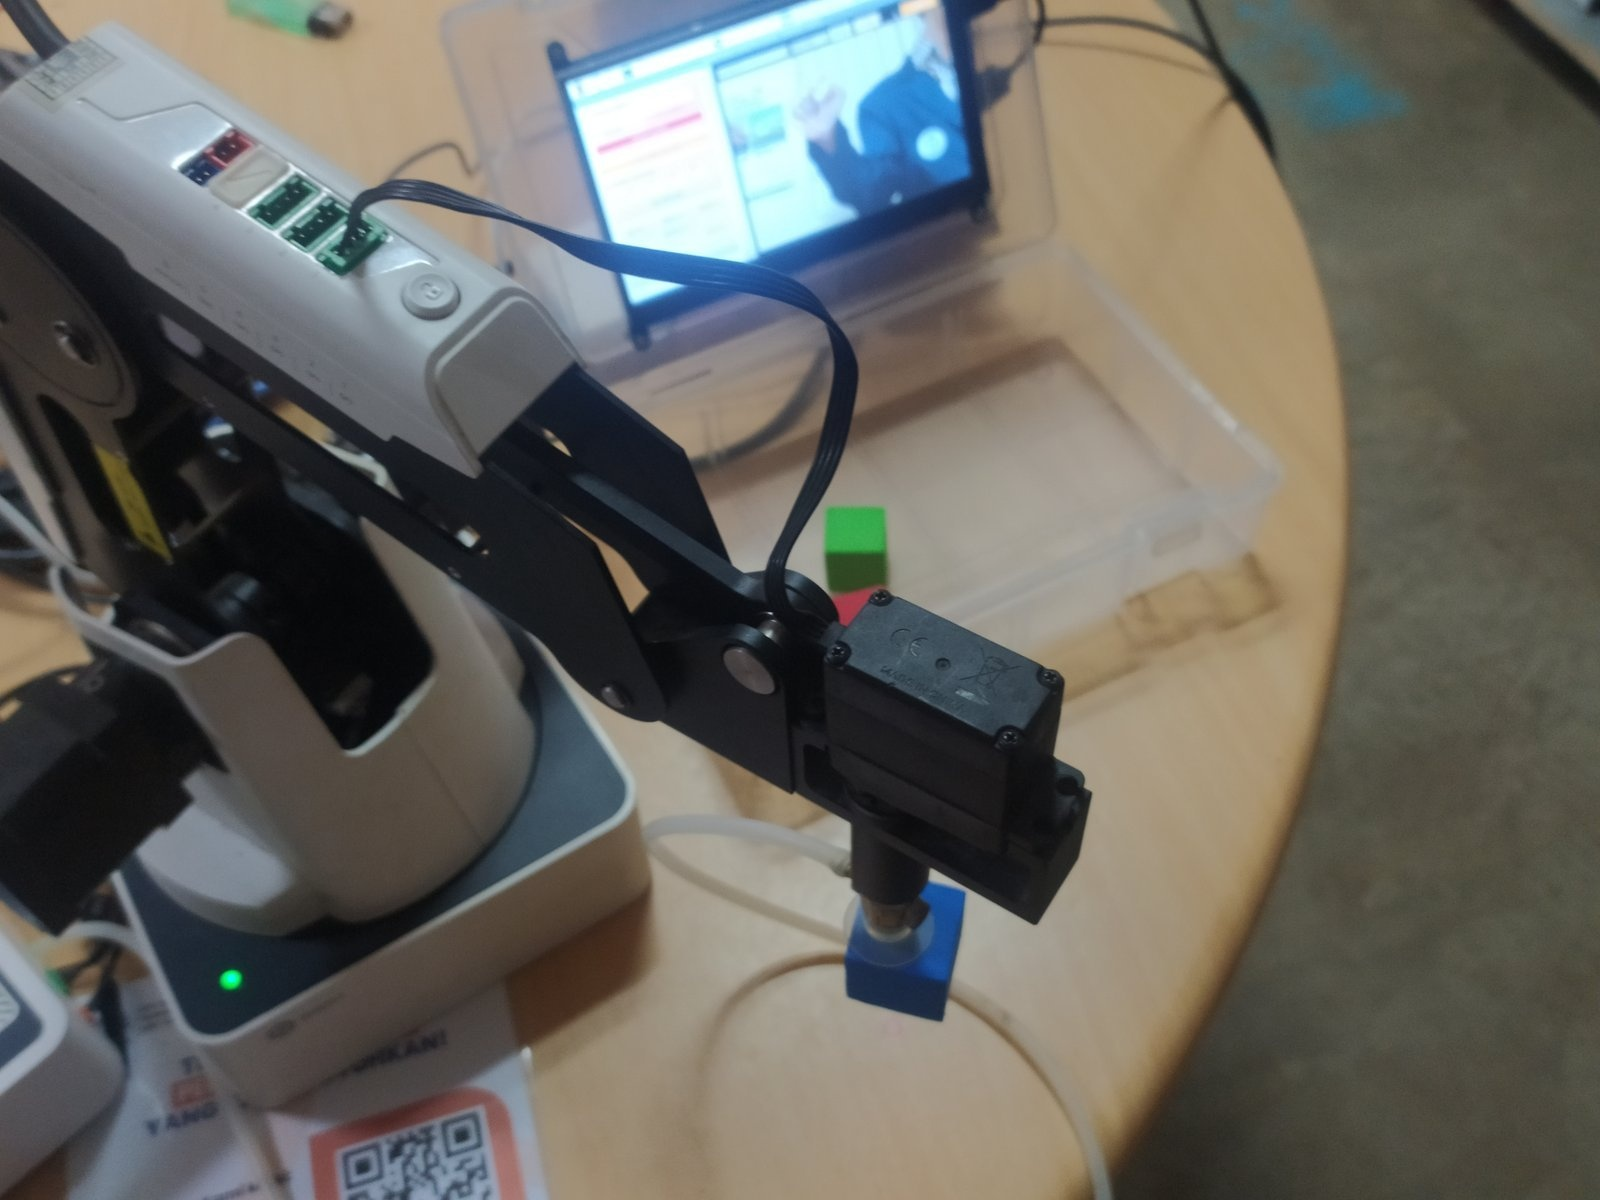
\includegraphics[width=\textwidth]{Gambar/Gambar6_17_manipulator_dobot_suction1.jpg}
        \caption{Manipulator Dobot dan Suction Cup (Sudut 1)}
        \label{fig:app_6_17}
    \end{subfigure}
    \caption{Dokumentasi Manipulator Dobot Magician}
\end{figure}

\begin{figure}[htbp]
    \centering
    \begin{subfigure}[b]{0.48\textwidth}
        \centering
        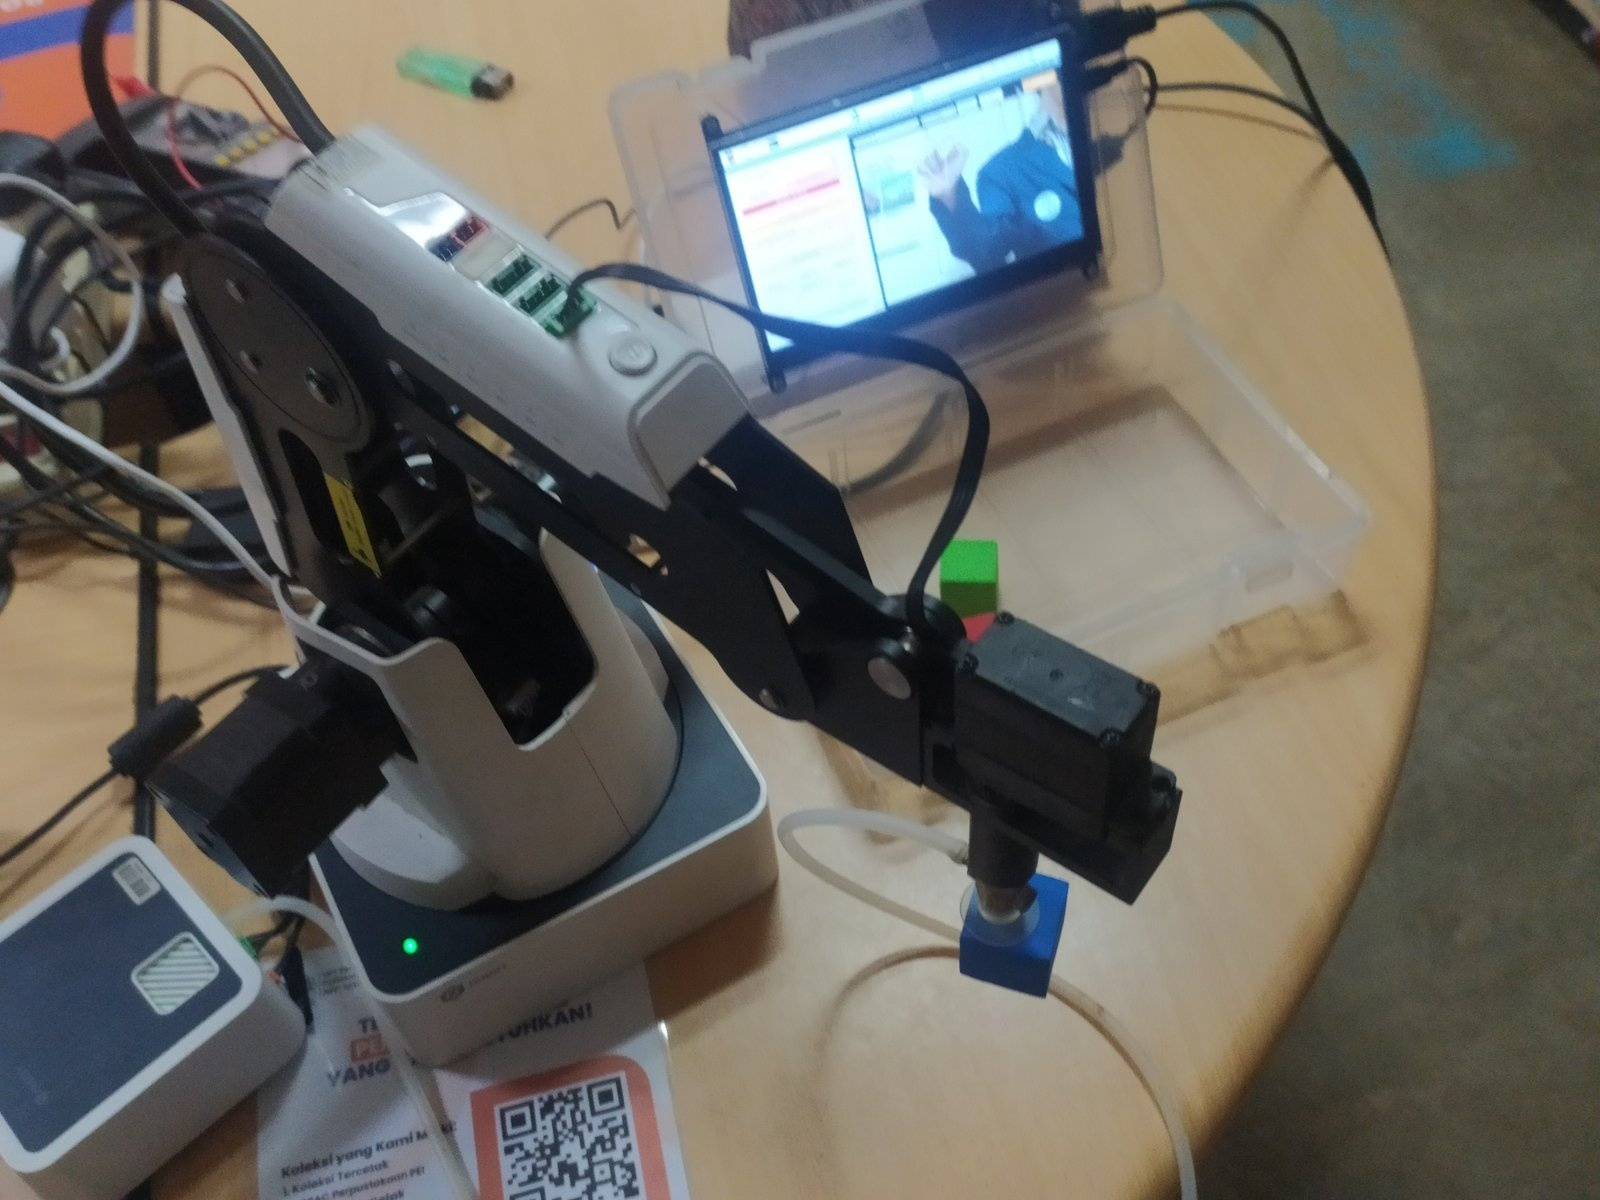
\includegraphics[width=\textwidth]{Gambar/Gambar6_18_manipulator_dobot_suction2.jpg}
        \caption{Manipulator Dobot dan Suction Cup (Sudut 2)}
        \label{fig:app_6_18}
    \end{subfigure}
    \hfill
    \begin{subfigure}[b]{0.48\textwidth}
        \centering
        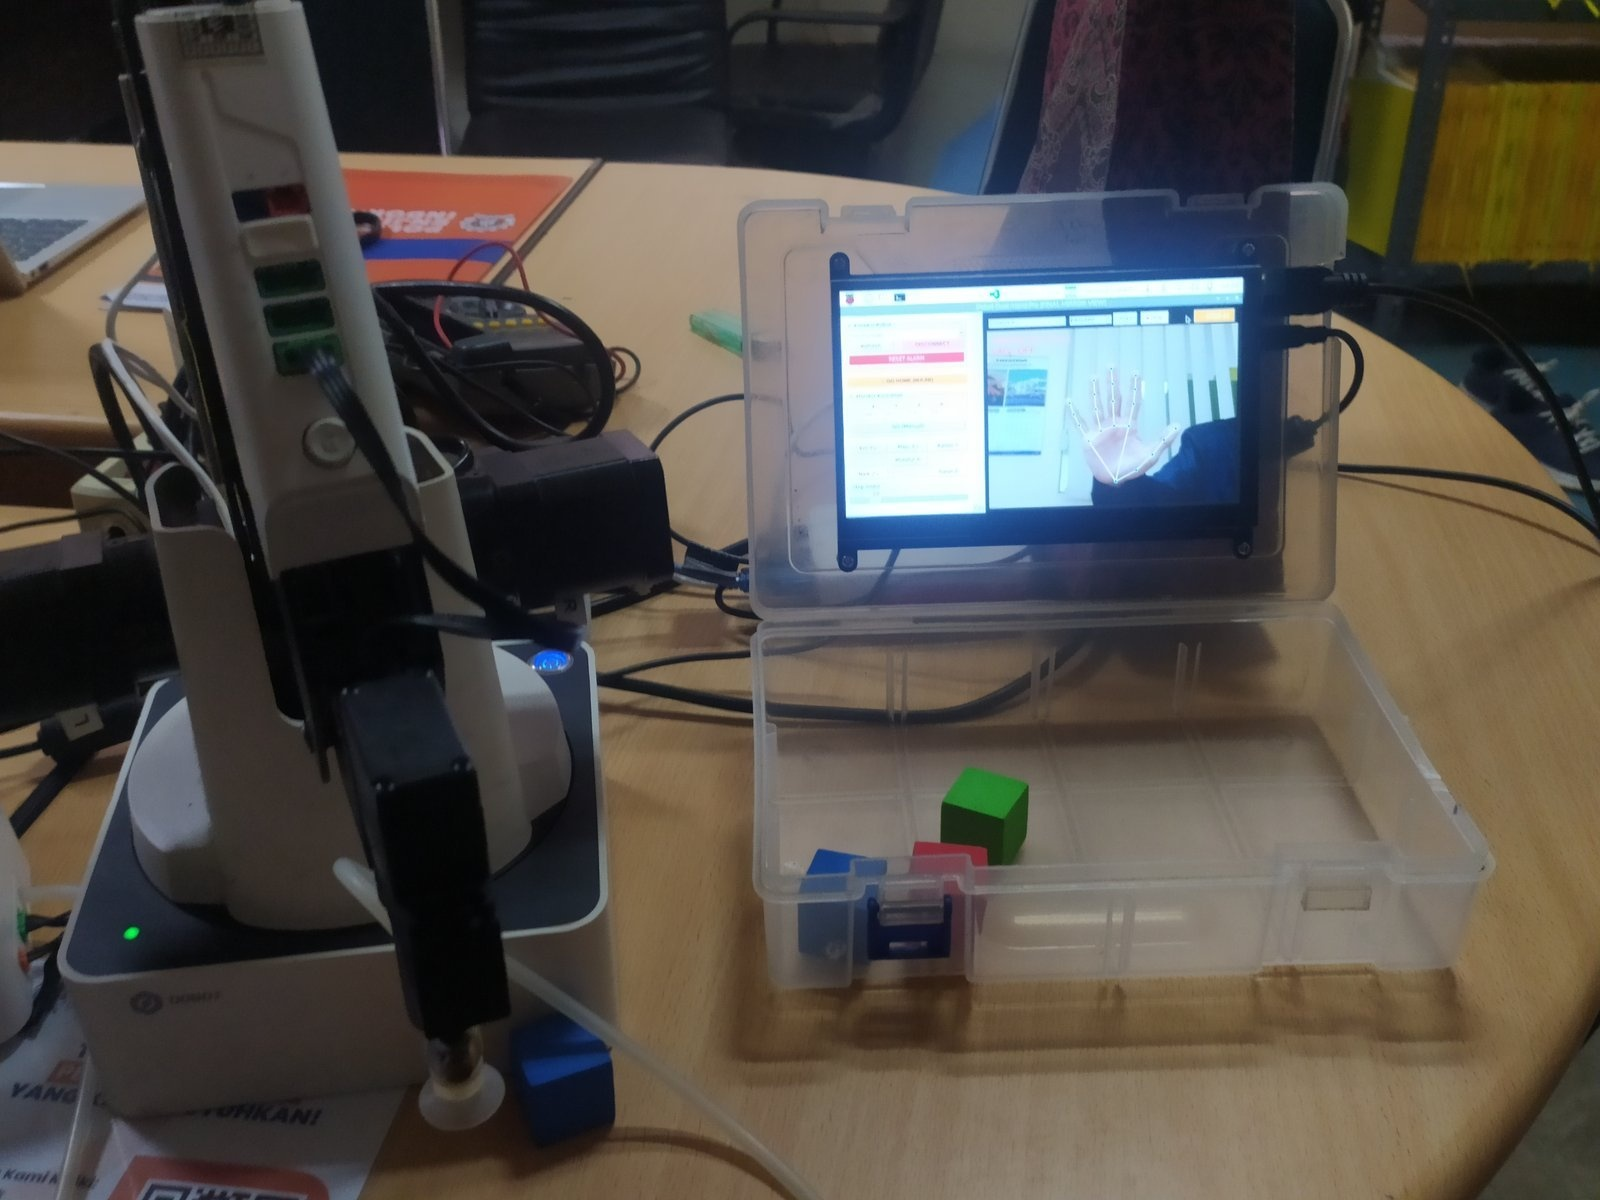
\includegraphics[width=\textwidth]{Gambar/Gambar6_19_manipulator_dobot_suction3.jpg}
        \caption{Manipulator Dobot dan Suction Cup (Sudut 3)}
        \label{fig:app_6_19}
    \end{subfigure}
    \caption{Pengujian Efektor Akhir Suction Cup Dobot Magician}
\end{figure}
